\documentclass[a4paper]{article}

\renewcommand{\labelenumii}{\theenumii}
\renewcommand{\theenumii}{\theenumi.\arabic{enumii}.}

\usepackage{fullpage} % Package to use full page
\usepackage{parskip} % Package to tweak paragraph skipping
\usepackage{tikz} % Package for drawing
\usepackage{amsmath}
\usepackage{amssymb,amsthm}
\usepackage{mathtools}
\usepackage{hyperref}
\usepackage{enumitem}
\usepackage{mathtools}
\usepackage{empheq}
\usepackage{amsfonts}
\usepackage{gensymb}
\usepackage{float}
\usepackage{subcaption}
\usepackage{placeins}
\usepackage{graphicx}


\newcommand*\widefbox[1]{\fbox{\hspace{2em}#1\hspace{2em}}}
%======================================== Title===========================================
\newcommand{\horrule}[1]{\rule{\linewidth}{#1}} 	% Horizontal rule
\title{
		\vspace{-0.6in} 	
		\usefont{OT1}{bch}{b}{n}
		\normalfont \normalsize \textsc{University of California Santa Cruz} \\ [10pt]
		\horrule{0.5pt} \\[0.4cm]
		\huge CMPE264 Project 2: Sweeping Plane Stereo \\
		\horrule{2pt} \\[0.5cm]
}
\author{
		\normalfont 								
        Aaron Hunter\\  Carlos Espinosa\\[-3pt]		\normalsize
}
%====================================Begin document=======================================
\begin{document}
\maketitle
%====================================Introduction=======================================
\section{Introduction}
In this report we document the process of generating a depth map of a scene by taking two images from different points of view.  To calculate the depth we triangulate between points that are visible in both images.  To perform the triangulation, however, we must determine both the relative camera orientations as well as the intrinsic camera parameters.  

The camera model (i.e., the intrinsic camera parameters) is developed through a calibration of a known target (in this case a checkerboard image) done in part 1. 

To find the relative camera pose we first need to capture two images of the same scene from different vantage points.  In Part 2 we construct a scene that comprised several different parallel planes with distinctive features. It is important to ensure that both images are translated and rotated enough to generate a large enough disparity between the images but still captures the same scene.  If the distance and rotation is too great, however, the homography applied to the images appears very distorted and doesn't provide a useful depth map.  

The relative orientation of the two cameras, known as the relative camera pose, is composed of the distance between the optical centers of the two camera positions and the relative orientation of the optical axis. This is performed in Part 3. The distance between the optical centers is known as the baseline and the orientation of the optical axes is a rotation matrix which is composed of the rotations around three orthogonal axes. To find the relative camera pose, we use functions in the OpenCV library to identify features common to both images.  We then use a matching function that determines the quality of the features, in other words, the confidence that both points actually correspond to a given surface point in the world.  Once identified we use another OpenCV function to determine the Essential Matrix, which relates the points in one camera reference frame to the other.  To confirm the fit we project the points found in one image onto the points found on the other image. If they coincide closely then we can have confidence in the determination of the relative camera pose.  

Finally, in Part 4 we implement the sweeping-stereo approach to calculating a depth map.  This is done by determining the depth of each feature point using the relative camera pose.  We then calculate the minimum and maximum depth in the scene and divide the three dimensional volume into 20 discrete planes spanning the depth of the image. We then warp one image using the plane parameters to generate the homography that translates a planar image in one reference system to the other. For each plane we determine which pixels coincide using an absolute difference between the images and finding the minimum value--where these pixels overlap with the reference image we can safely assign a depth to those pixels.  This is done for every pixel over all 20 warped images until the minimum is found. Finally, we convert these depths values into a gray scale eight bit integer and display a depth map.  Note the depth is relative to the baseline of the two vantage points.
%====================================Part 1=======================================
\section{Camera calibration}
In this section we perform the camera calibration by taking many (some websites recommend more than 20) images of a known target.  We selected a fixed focal length lens to minimize any possible variations between the calibration images and the final scene images. The camera used is a Fuji X-E1 with a 60mm prime lens set to f/8.  The target is a 6x9 checkerboard target taken from OpenCV.org, taped it to a flat board and we captured images of it at multiple orientations.  The images are shown in fig(\ref{fig:chkbd}) below.
 \begin{figure}[htb!]
    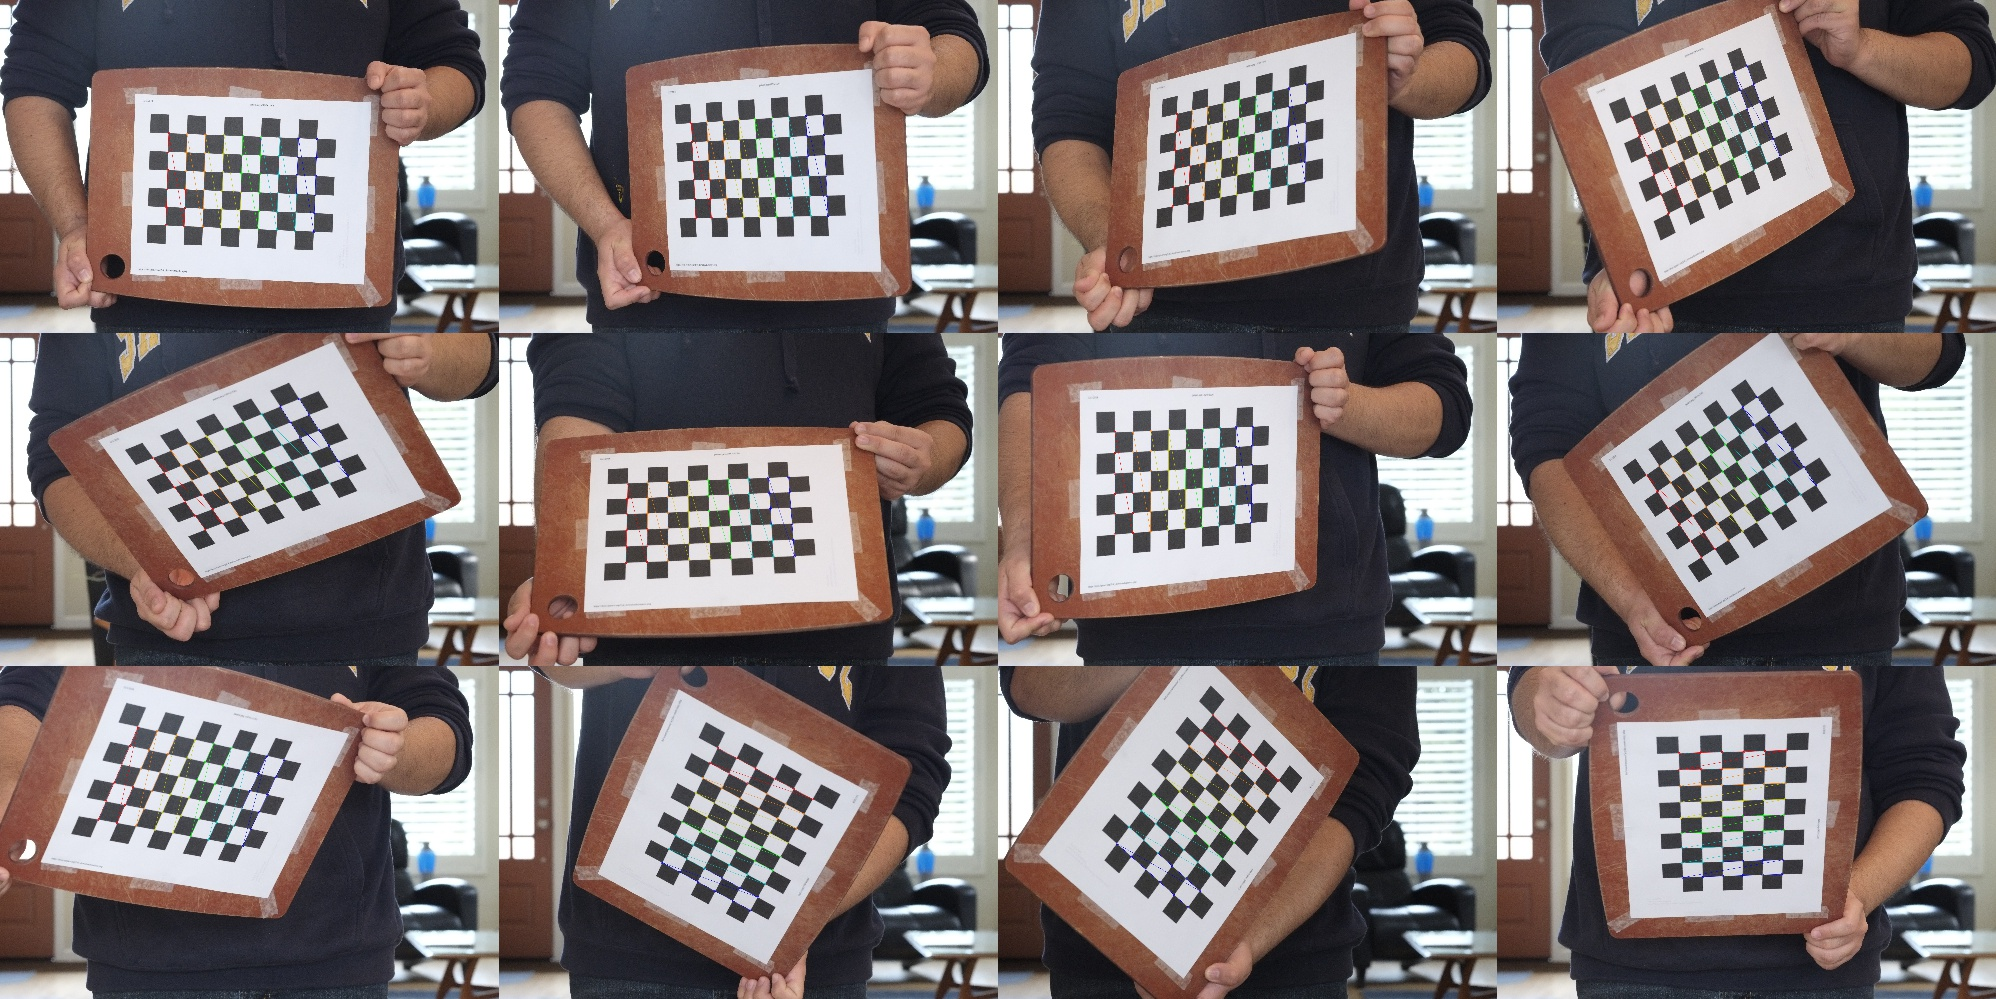
\includegraphics[width=\textwidth]{../CamCal}
    \caption{Calibration Images of 6x9 checkerboard pattern.}
    \label{fig:chkbd}
\end{figure}
\FloatBarrier
The intrinsic matrix is calculated by using the \verb|cv2.calibrateCamera()| function which attempts to find all 54 internal corners of the target in every image.  It then estimates the best fit for all the intrinsic camera parameters stored in the intrinsic matrix.  The general form of the intrinsic matrix is:
\begin{align*}
	\begin{bmatrix}
		f & 0 & c_x\\
		0 & f & c_y\\
		0 & 0 & 1
	\end{bmatrix}
\end{align*}
The algorithm also estimates the radial distortion parameters of the lens and presented at a matrix of polynomial values.  The function also returns the estimation error in pixels.  The  intrinsic camera matrix and radial distortion parameters returned by the algorithm are shown below.  Note that the focal length found is accurate only to scale since we didn't use a measurement of the locations of the checkerboard corners, rather just the number of corners. The center of the sensor (downscale somewhat from the highest resolution the camera is capable of) is close however, at (1304,743). The camera matrix is:
\begin{align*}
	\begin{bmatrix}
             6.95471201e+03 & 0.00000000e+00  & 1.30414502e+03\\
            0.00000000e+00  & 6.95274412e+03  & 7.42329190e+00\\
            0.00000000e+00  & 0.00000000e+00  & 1.00000000e+00
         \end{bmatrix}
\end{align*}
The radial distortion coefficients are:
\begin{align*}
	\begin{bmatrix}
		-7.03044644e-02 & 2.40329209e+00 &  -5.12362432e-03 & 1.70607379e-03  &  -7.16979565e-04
	\end{bmatrix}
 \end{align*}
 The reprojection mean square error is found to be approximately 0.250 pixels.
 \FloatBarrier

%====================================Part 2=======================================
\section{Scene Images}
Now that we have our camera calibration we need to take images of a scene.  We worked with a few different ones, eventually using one that presented multiple parallel planes that could be resolved into discrete depths.  We also tried to collect objects with identifiable texture.  One interesting feature of our scene is that it has a very contrasty natural stone. This actually proved to be not as beneficial as we expected and created interesting artifacts in the final depth map of the scene.  The two images are shown in figs(\ref{fig:sn1},\ref{fig:sn2}).

\begin{figure}
    \centering
    \begin{subfigure}[b]{0.45\textwidth}
        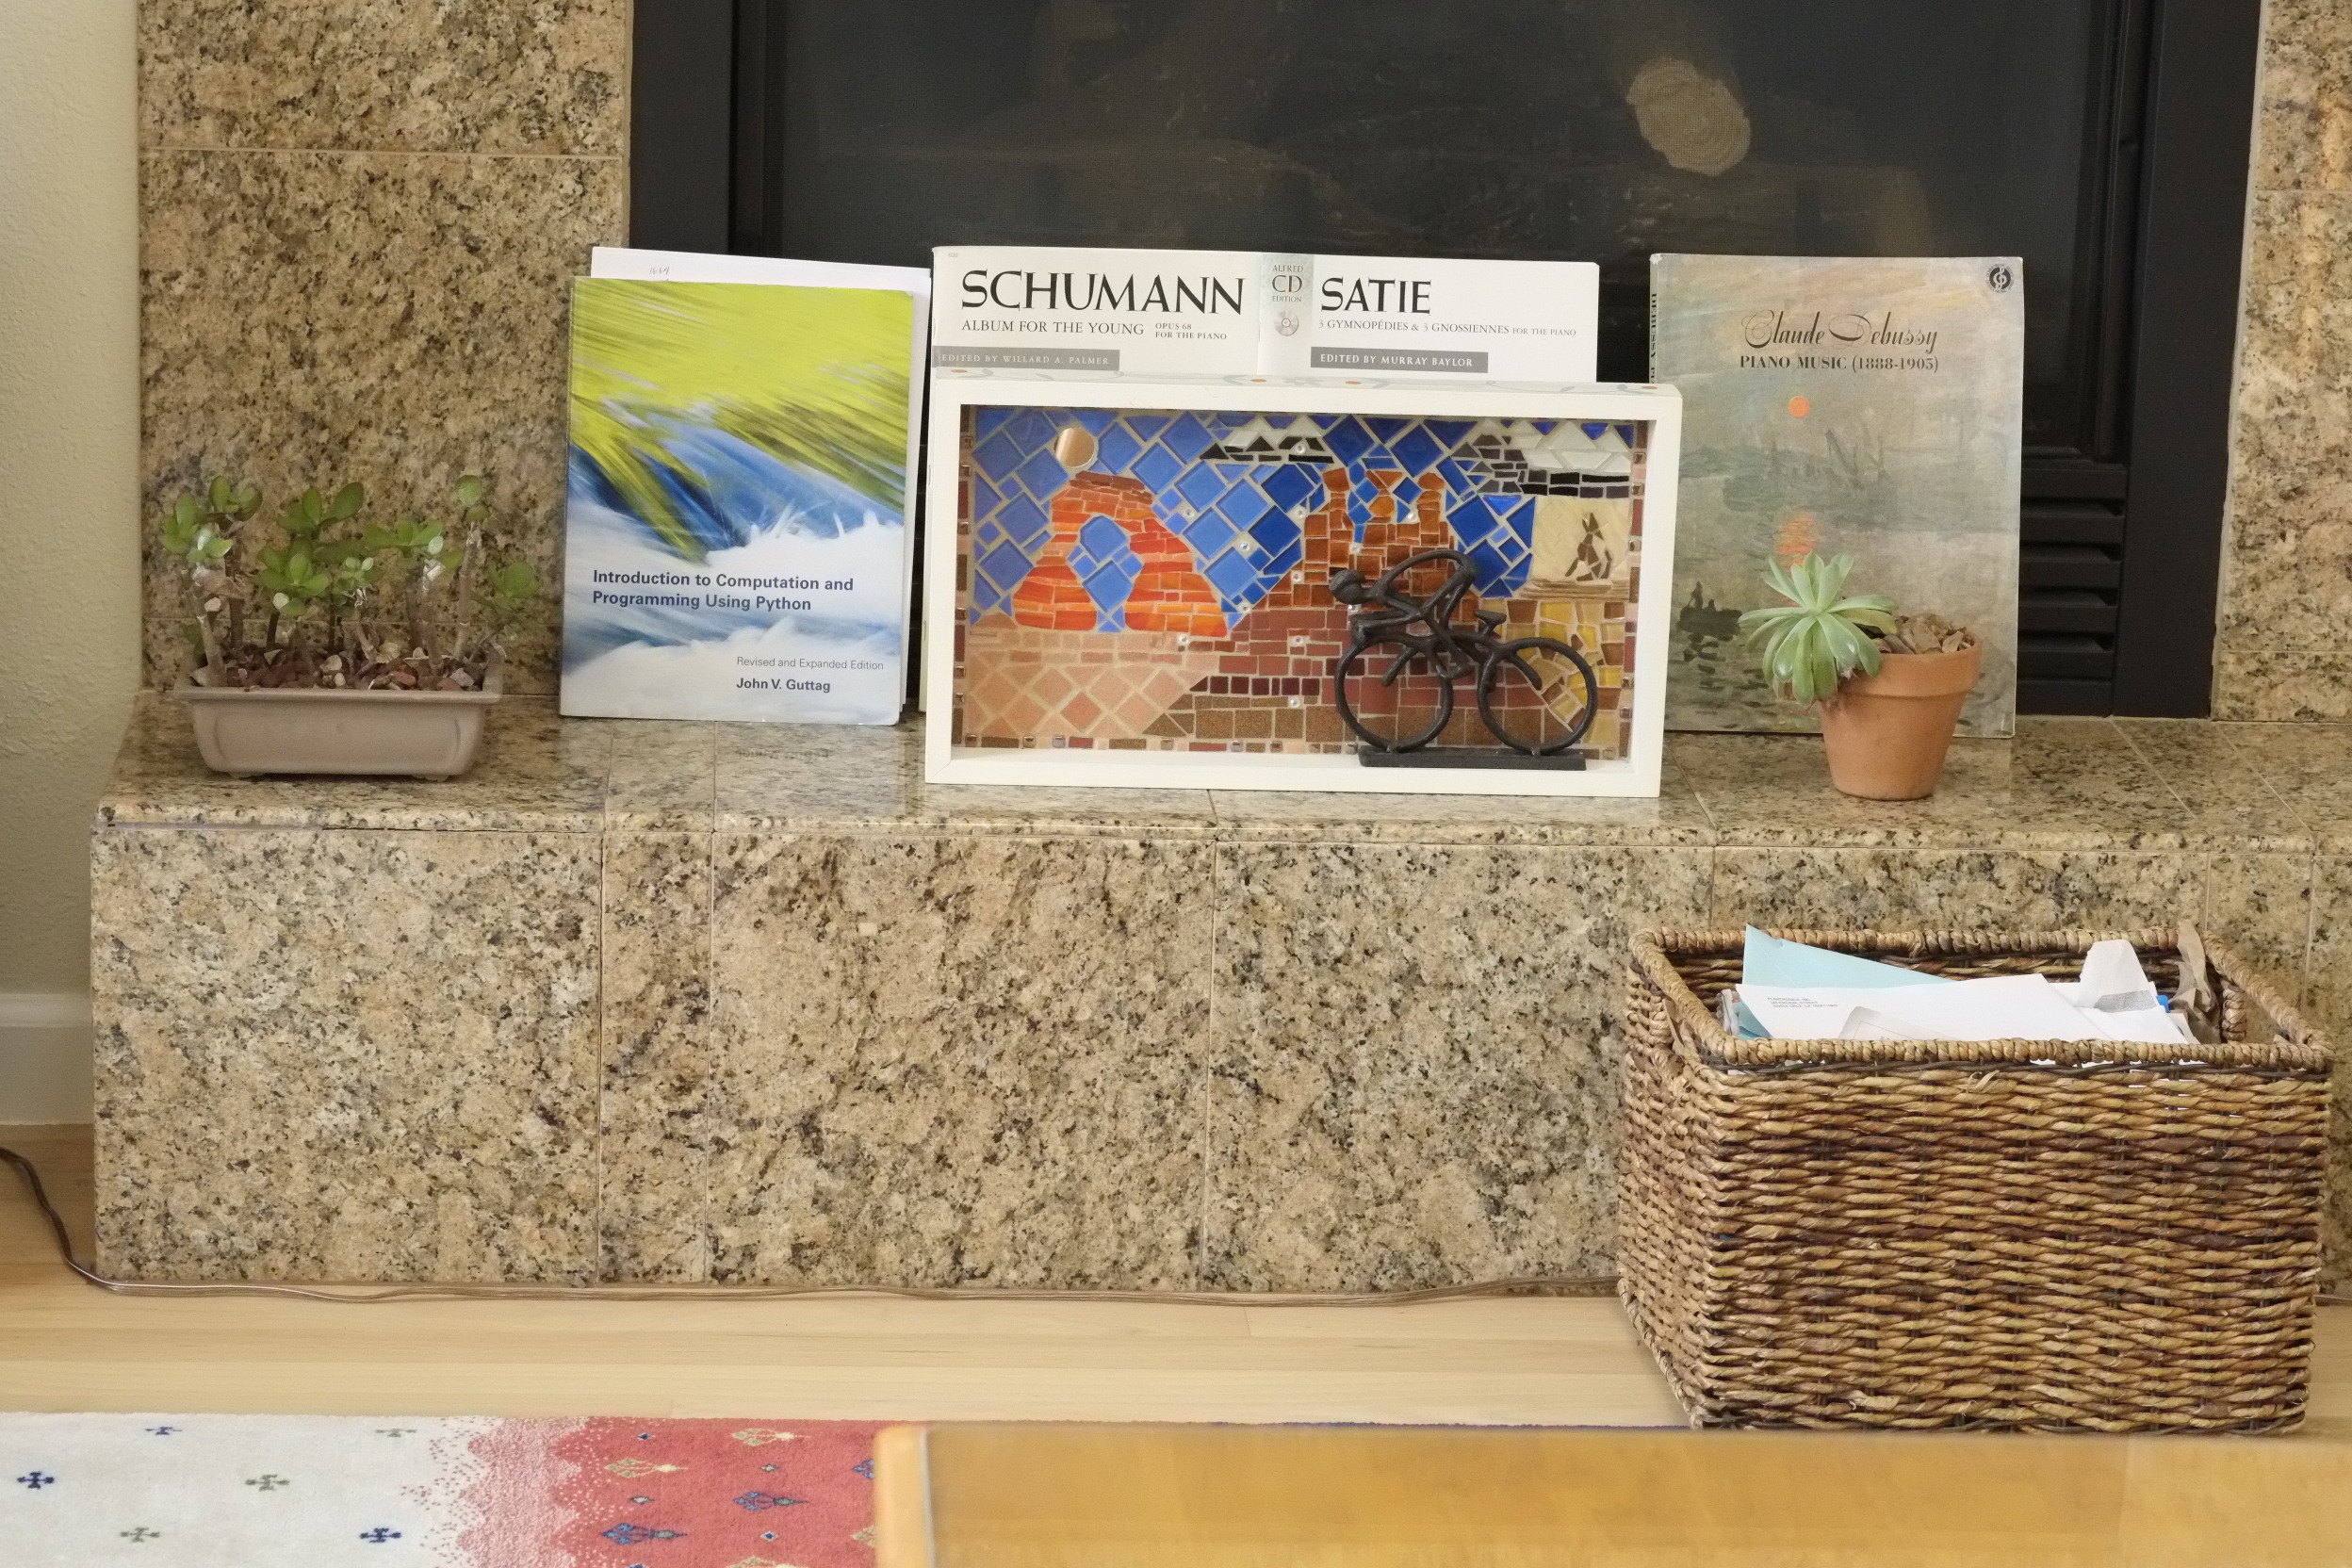
\includegraphics[width=\textwidth]{../Scene/_DSF1768.JPG}
        \caption{First scene image}
        \label{fig:sn1}
    \end{subfigure}
    \begin{subfigure}[b]{0.45\textwidth}
        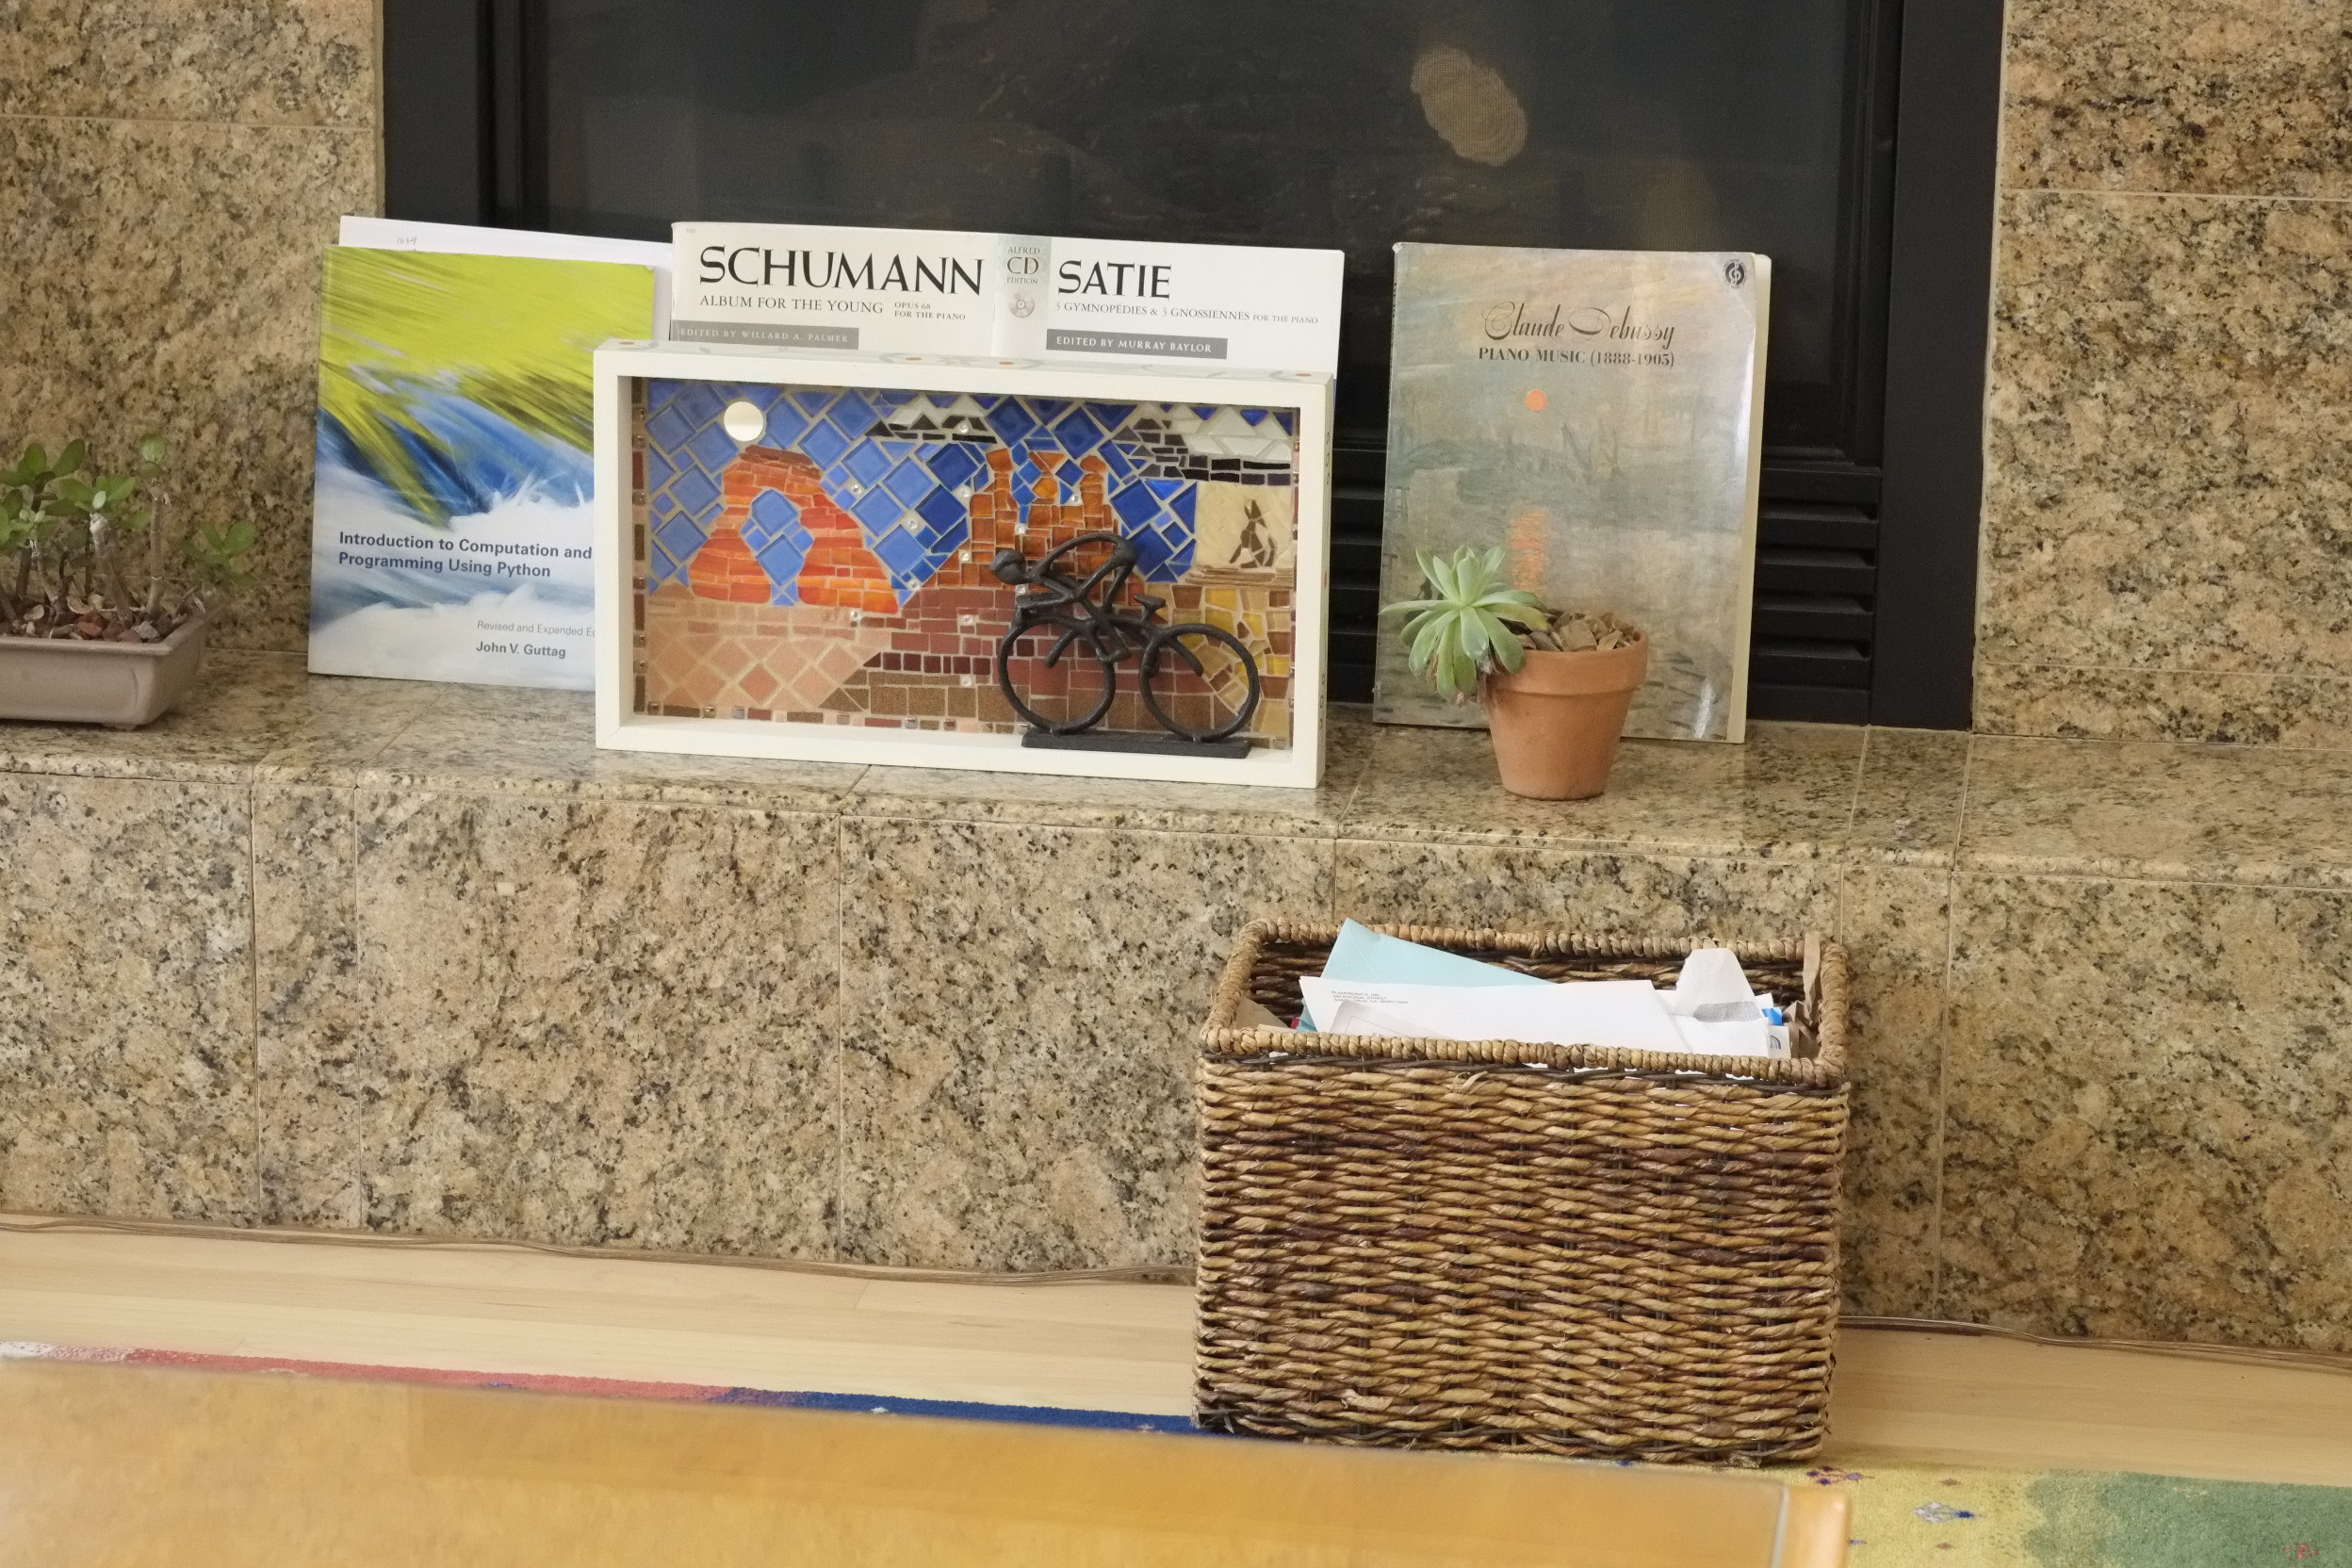
\includegraphics[width=\textwidth]{../Scene/_DSF1769.JPG}
        \caption{Second scene image}
        \label{fig:sn2}
    \end{subfigure}
\end{figure}

\FloatBarrier

%====================================Part 3=======================================
\section{Relative Camera Pose}
After taking two reasonable images of the same scene, the next step is to account for the distortion inherent in the camera by employing the \verb|undistortPoints()| function on both images.  Once they have been corrected we find feature points that exist in both images.  The OpenCV function \verb|sift.detectAndCompute()| is used to identify good candidate feature points in both images.  The points are then sent to a matching function, in this case \verb|cv2.FlannBasedMatcher()|.  This function generates a distance feature that is used to discriminate between good features. We explored several tutorials within OpenCV documentation primarily the one on camera calibration. 

Armed with these feature points we can explore a few of them to determine epipolar lines that connect feature points in one image to the corresponding points in the other image.  To compute the epipolar lines we need first to determine the Fundamental matrix, which consists of the transformation matrix that converts pixels in one image to pixels in the other image.  The function \verb|cv2.findFundamentalMat()| takes the matched points and returns the Fundamental matrix.  This matrix is used to calculate the epipoles along with matching feature points.  Strictly speaking computing the epipoles is not used for computing the depth map, however, they are helpful by providing visual confirmation of successful feature point matches. A sample of our matching points connected by epipolar lines is shown in figs(\ref{fig:epi_a},\ref{fig:epi_b},\ref{fig:epi_c},\ref{fig:epi_d}) below.

\begin{figure}
    \centering
    \begin{subfigure}[b]{0.45\textwidth}
        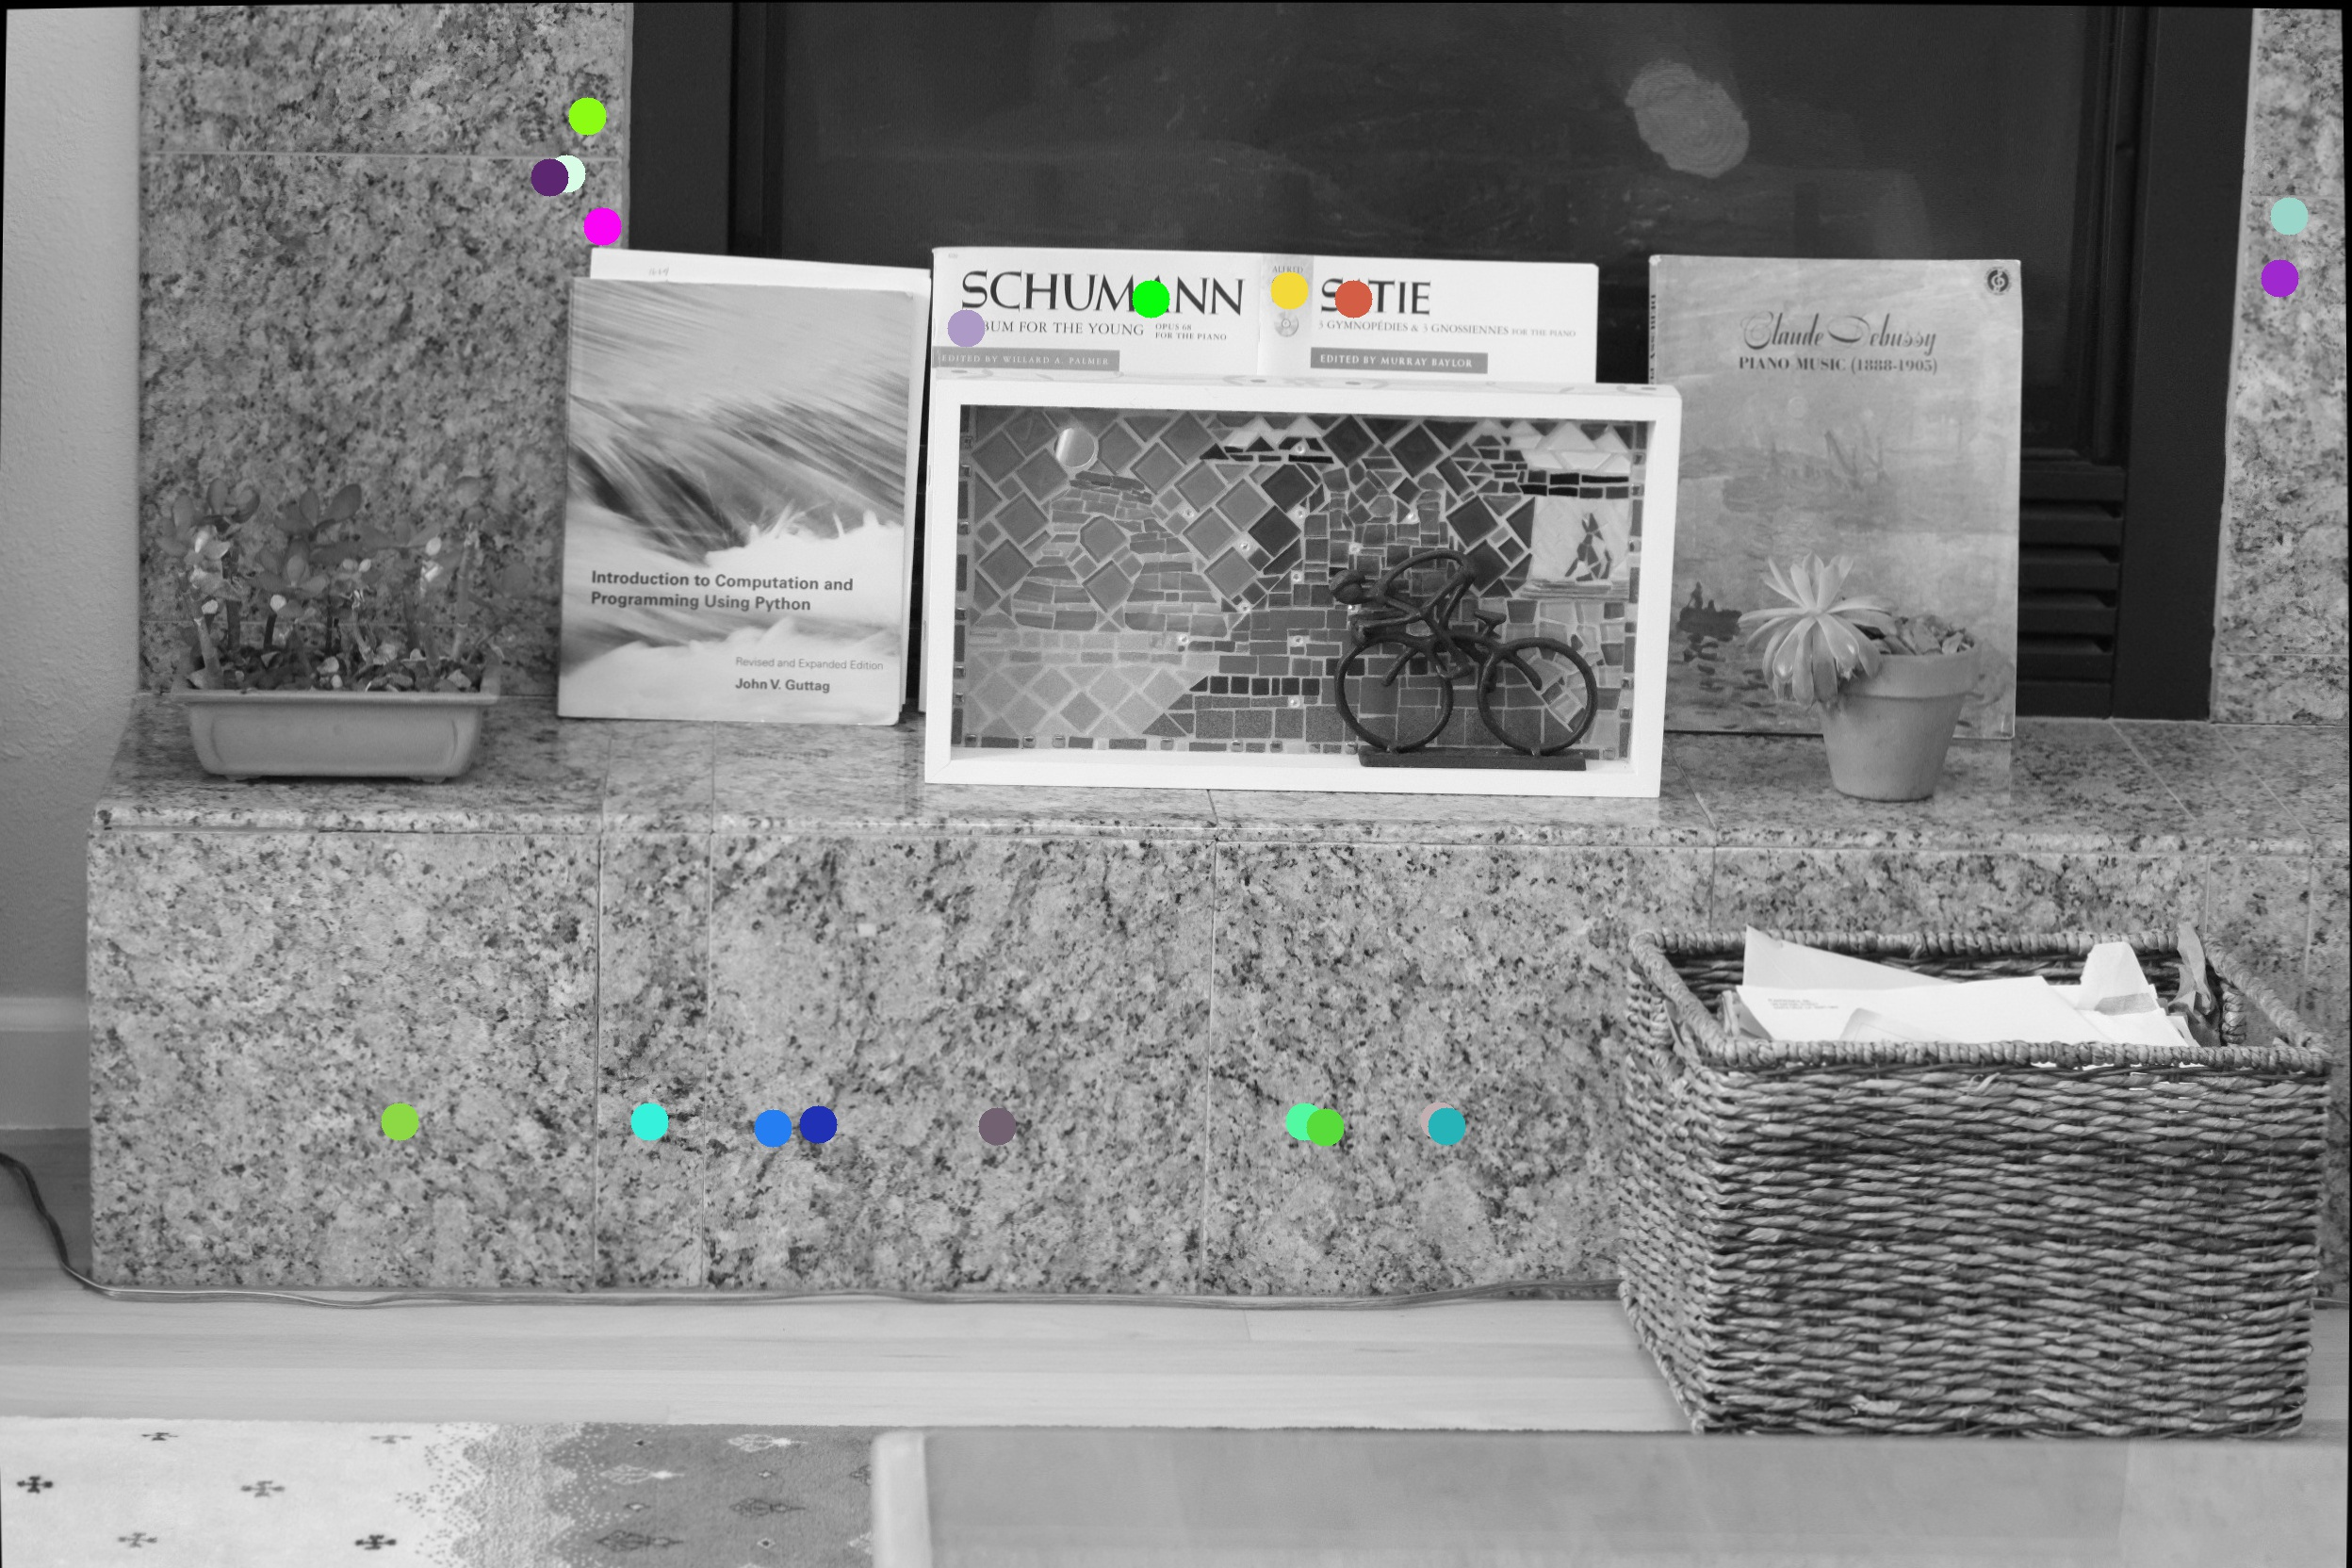
\includegraphics[width=\textwidth]{../epi2}
        \caption{Feature points in image 1.}
        \label{fig:epi_a}
    \end{subfigure}
    \begin{subfigure}[b]{0.45\textwidth}
        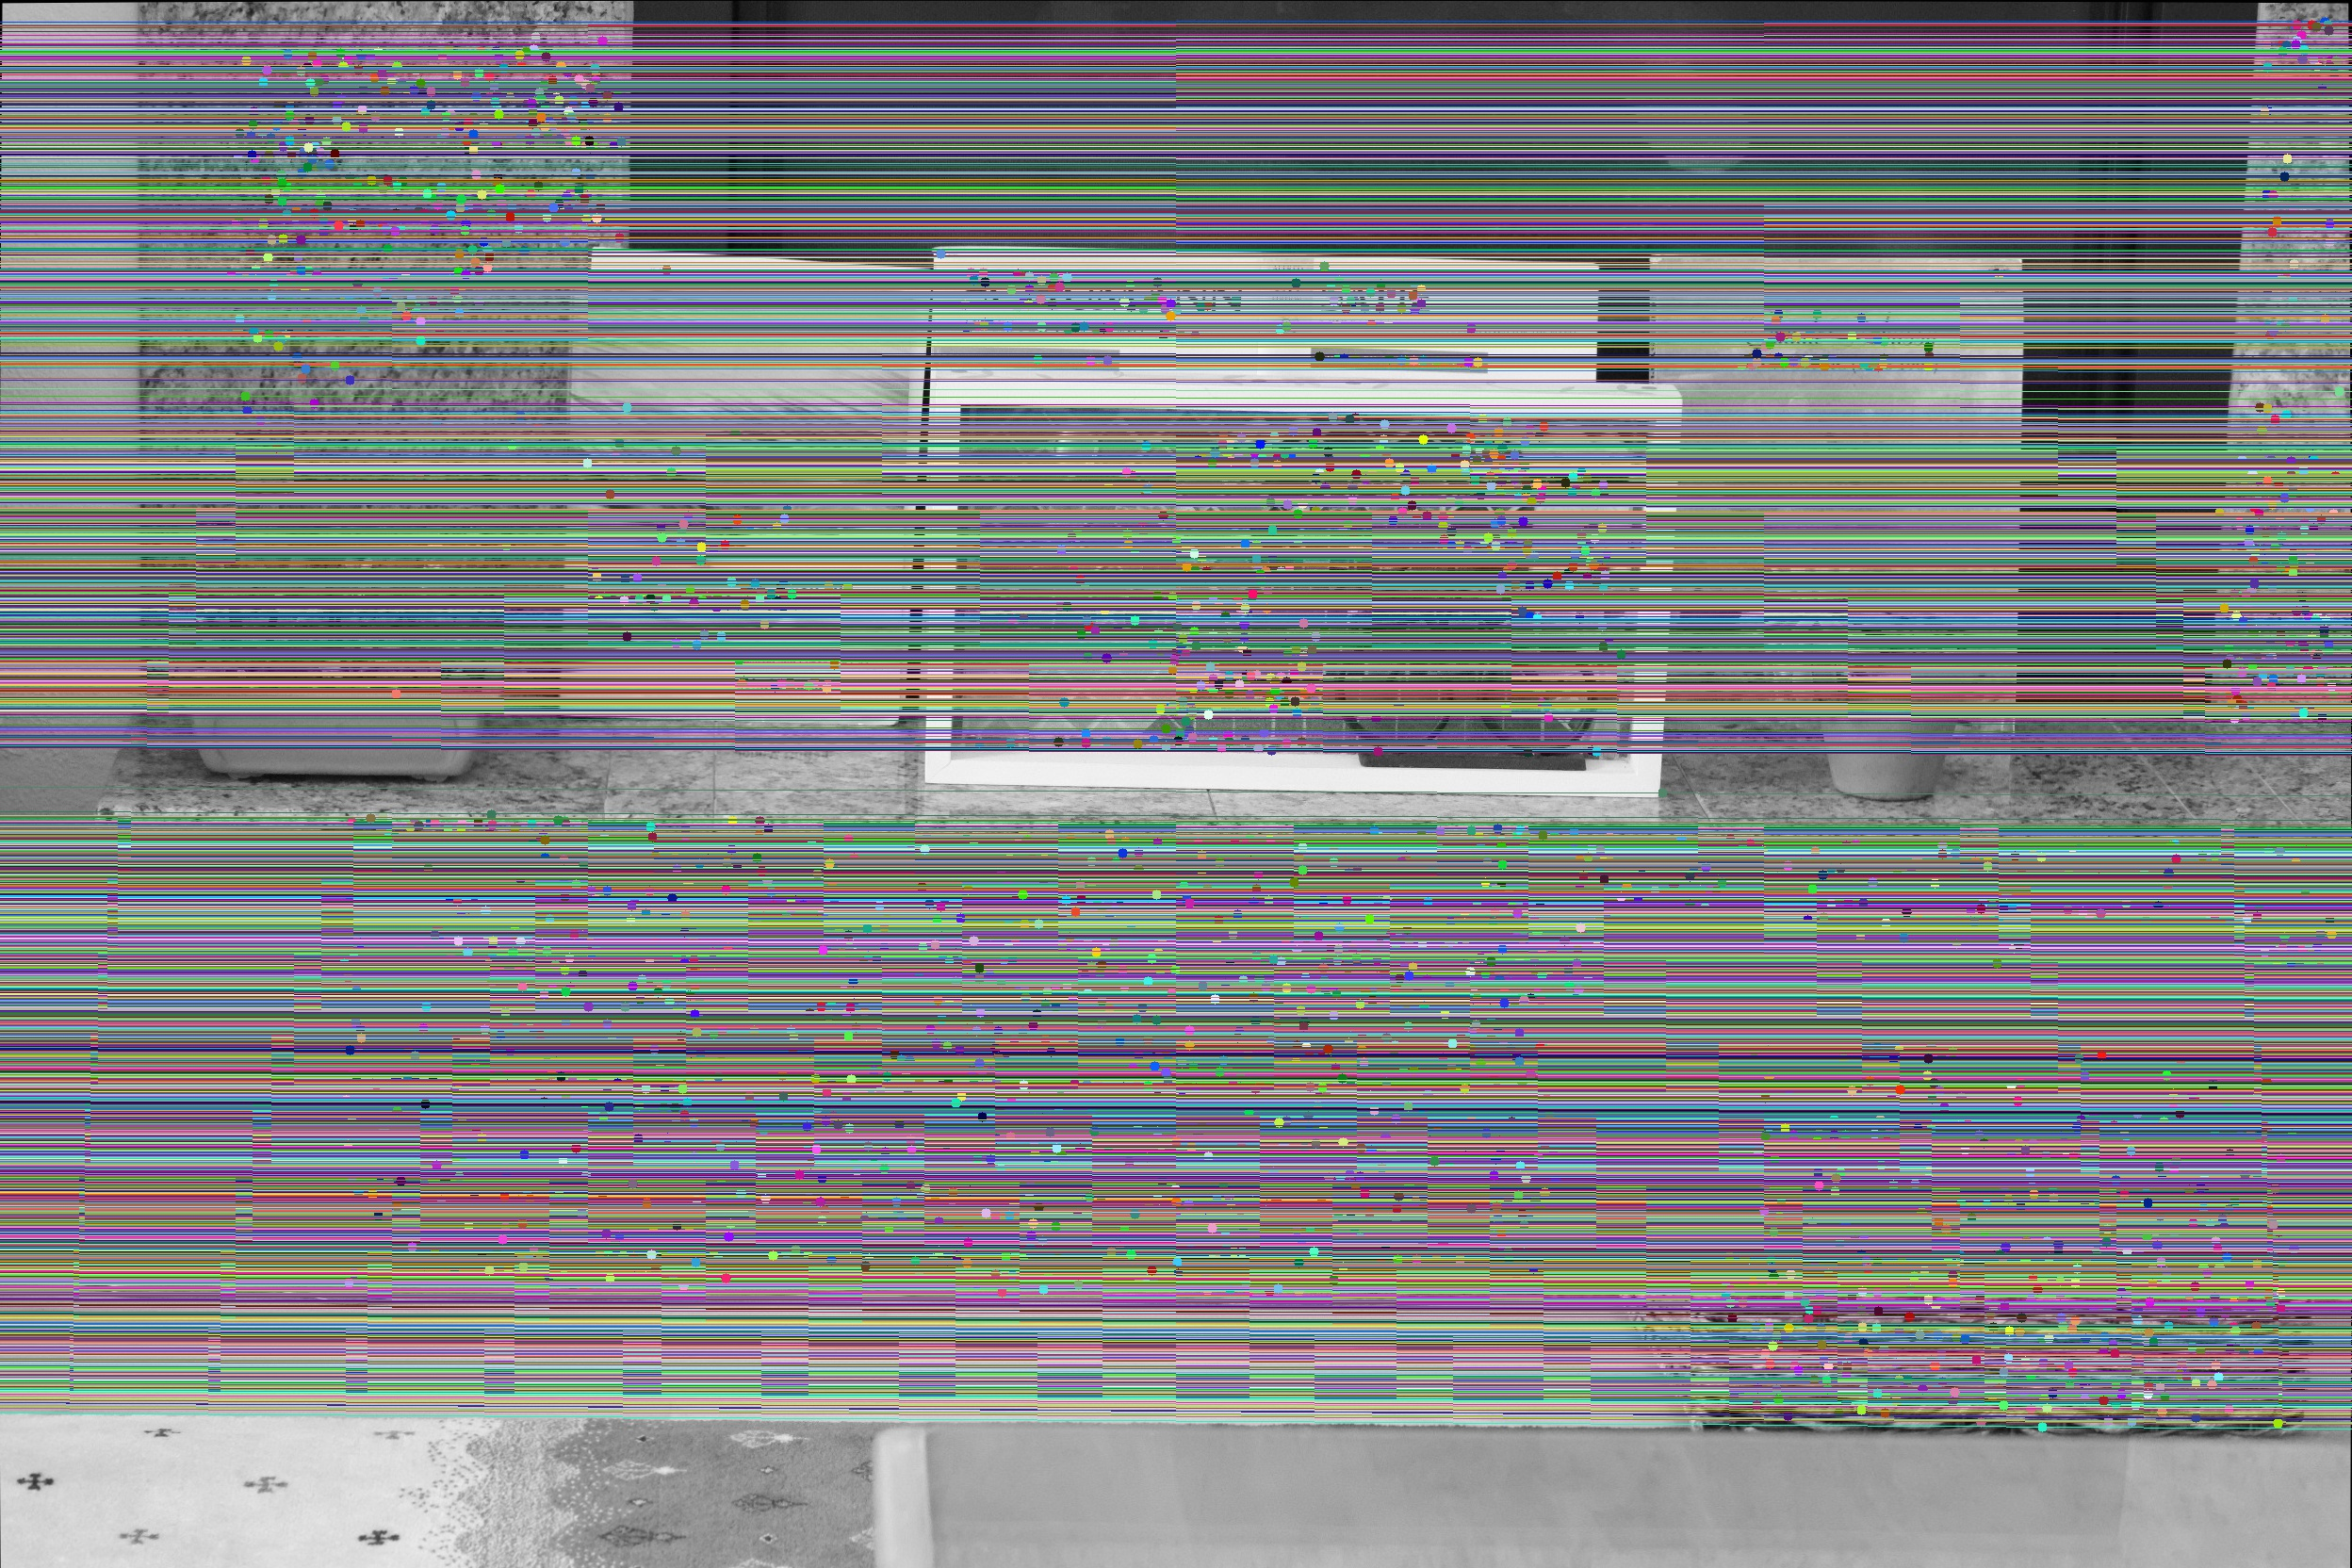
\includegraphics[width=\textwidth]{../epi1}
        \caption{Epipolar lines for the points in image 1.}
        \label{fig:epi_b}
    \end{subfigure}
\end{figure}

\begin{figure}
    \centering
    \begin{subfigure}[b]{0.45\textwidth}
        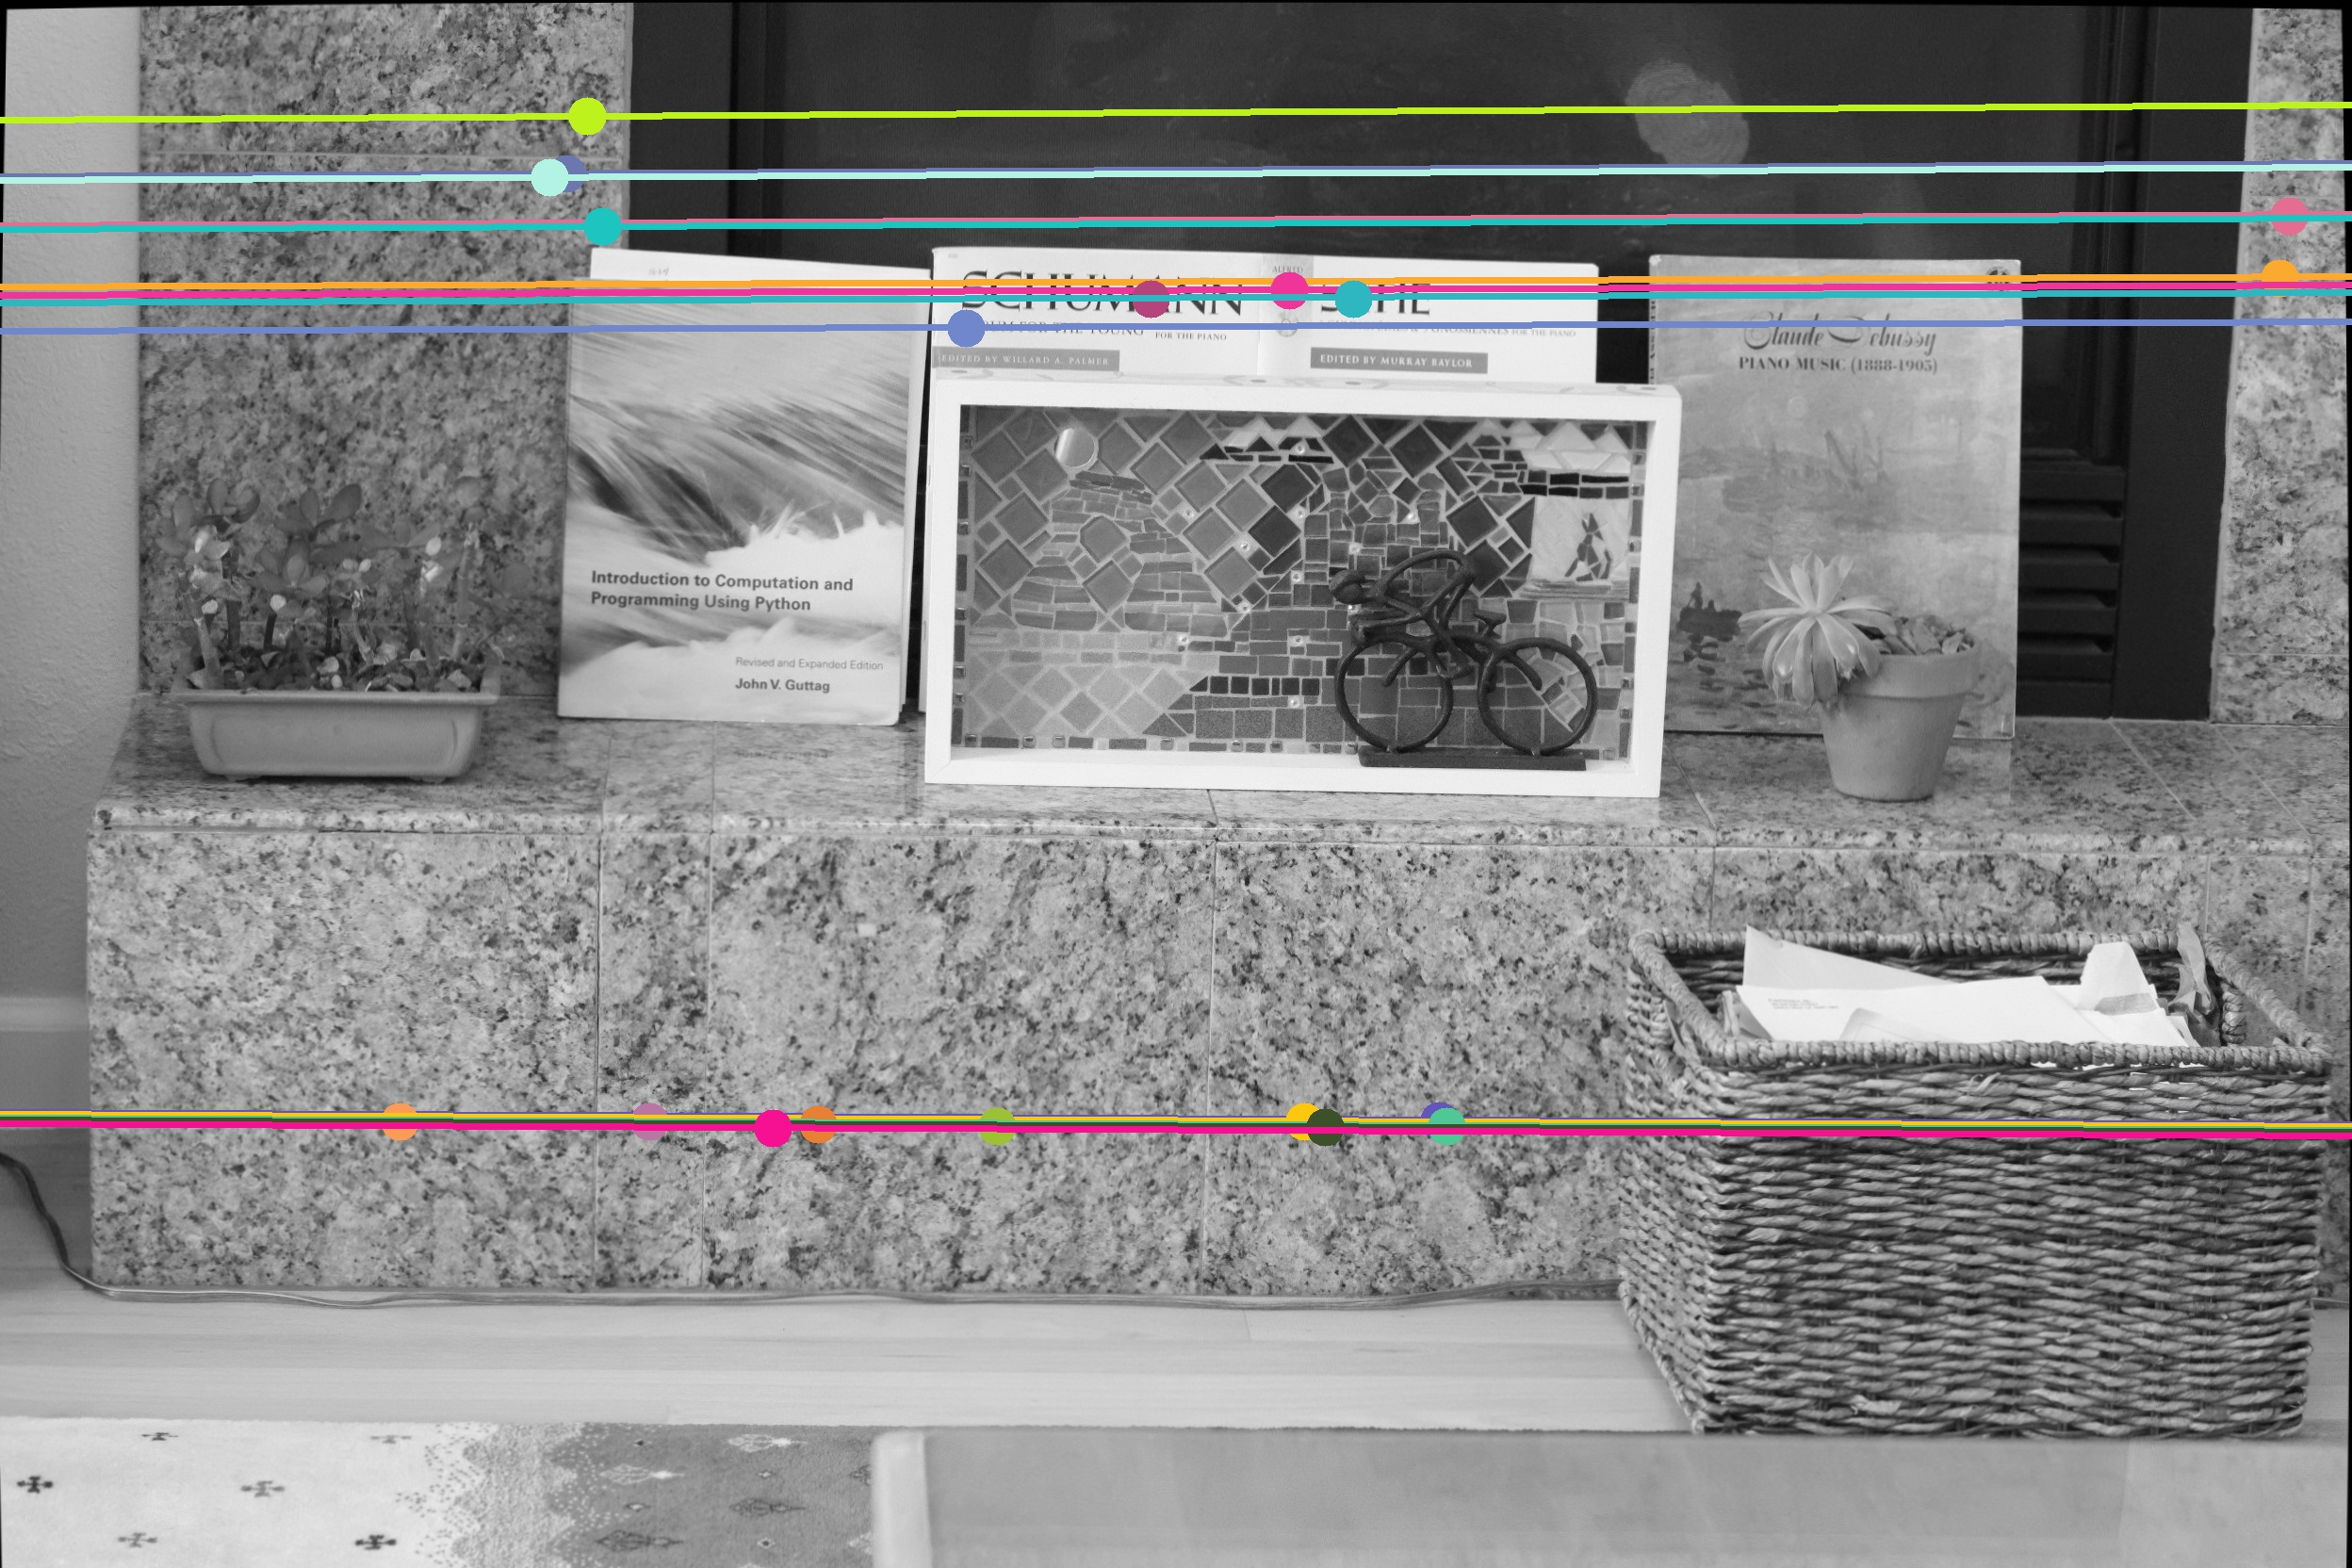
\includegraphics[width=\textwidth]{../epi3}
        \caption{Epipolar lines for the points in image 2.}
        \label{fig:epi_c}
    \end{subfigure}
    \begin{subfigure}[b]{0.45\textwidth}
        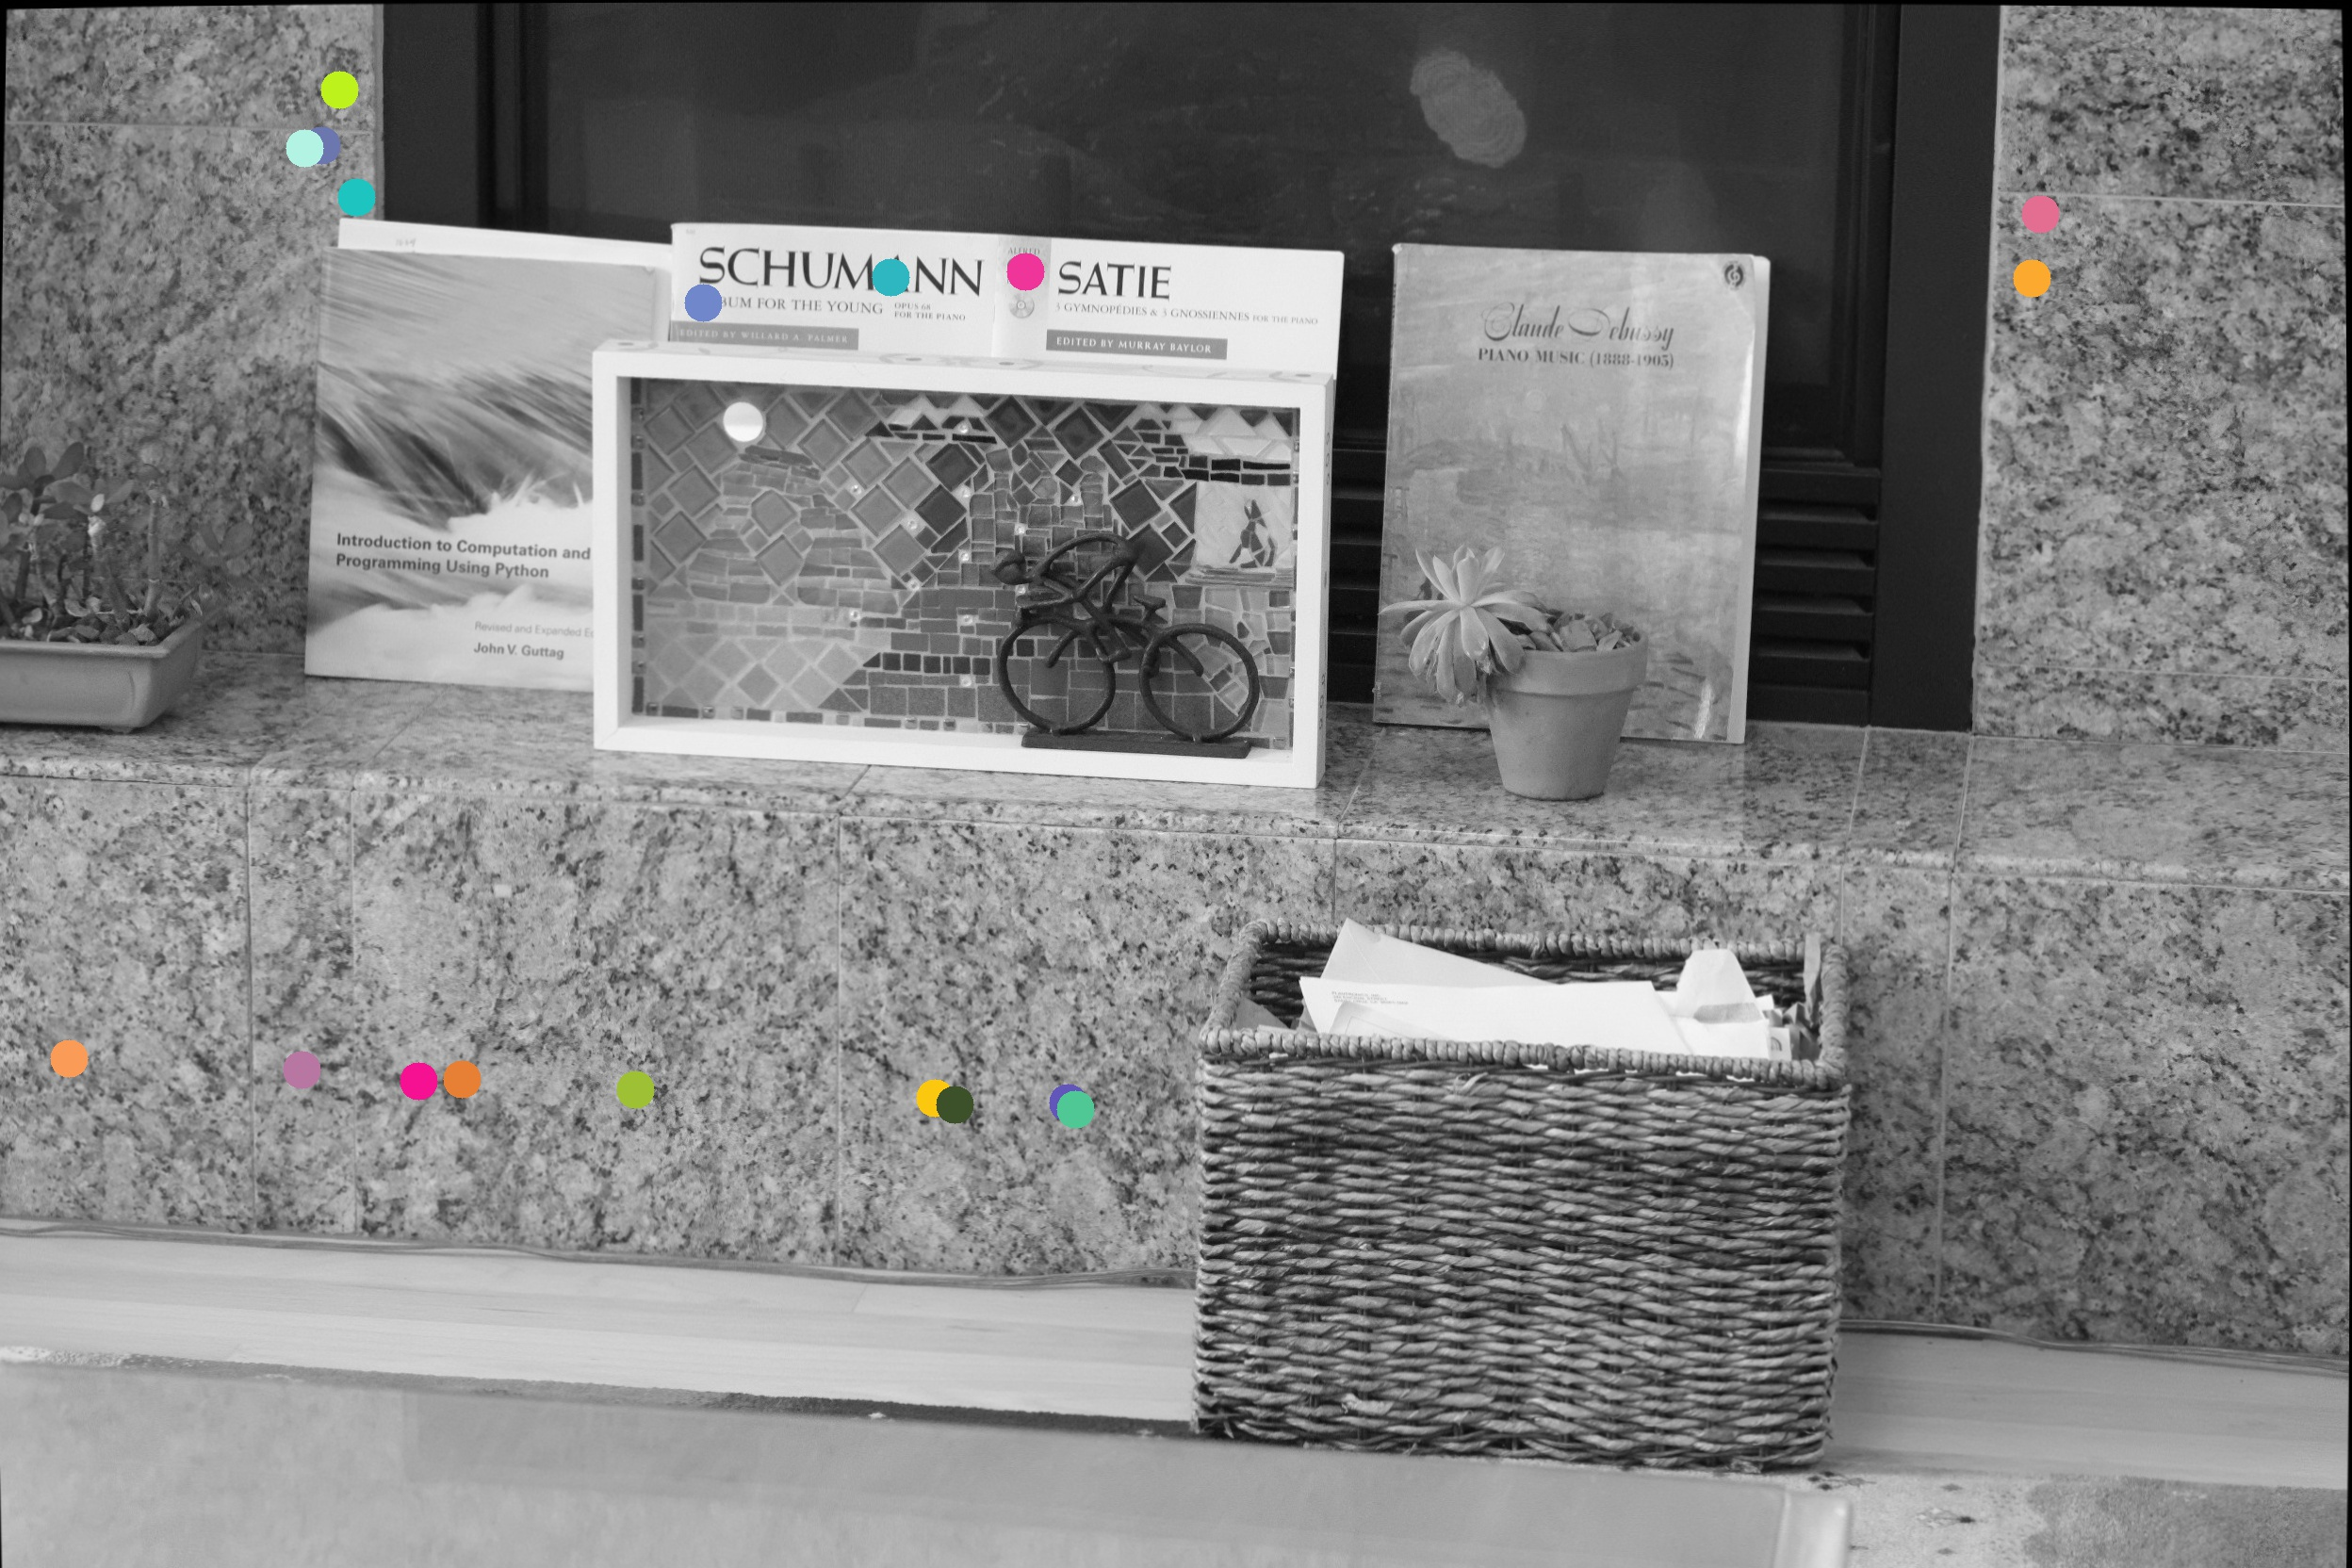
\includegraphics[width=\textwidth]{../epi4}
        \caption{Feature points in image 2.}
        \label{fig:epi_d}
    \end{subfigure}
\end{figure}

To determine the relative camera pose (the rotation matrix and translation vector) between the two cameras, we next calculate the Essential matrix which is transformation matrix that translates points in one camera centered reference frame to the other.  We employed the \verb|findEssentialMat()| function which takes parameters extracted from the intrinsic matrix that we found in Part 1.  From the Essential matrix it is possible to find the relative camera pose, however, it is ambiguous--it returns two possible rotation matrices and one translation vector, but we do not know which rotation matrix is correct, nor the sign of the translation vector.  To resolve this ambiguity we calculated the homogeneous (four-dimensional) points corresponding to our pixels by providing the \verb|triangulatePoints()| function with the four possible combinations.  This function takes as its input the camera pose information for both cameras.  We want the reference system to be centered on our first camera optical center, so we take its rotation matrix to be the identity matrix and the zero vector as its translation vector.  Only points that have positive z value are correct.  Those were associated with our second rotation matrix and positive translation vector.  The rotation matrix is therefore:
\begin{equation*}
	R _L^R= 
	\begin{bmatrix} 
	0.97625117 & 0.03161439 & -0.2143226\\
       -0.03292285 & 0.99945468 &  -0.00253737\\
        0.21412551 & 0.00953322 &  0.97675963
       \end{bmatrix}
\end{equation*} 
And the translation vector is:
\begin{align*}
	\bf{r}^R = 
	\begin{bmatrix} 
		0.99362709\\
               0.01693907\\
               0.11143728
	\end{bmatrix}
\end{align*}

Finally, we take the (homogenous) points in the camera 1 reference system and reproject the points onto the first image.  To project these points onto image 1, we need to convert twice from homogenous coordinates, then multiply by the intrinsic calibration matrix. These points are shown below in fig(\ref{fig:reproj}).  Of interest is the large number of feature points located in the natural stone also several distinct planes are visible.

 \begin{figure}[htb!]
    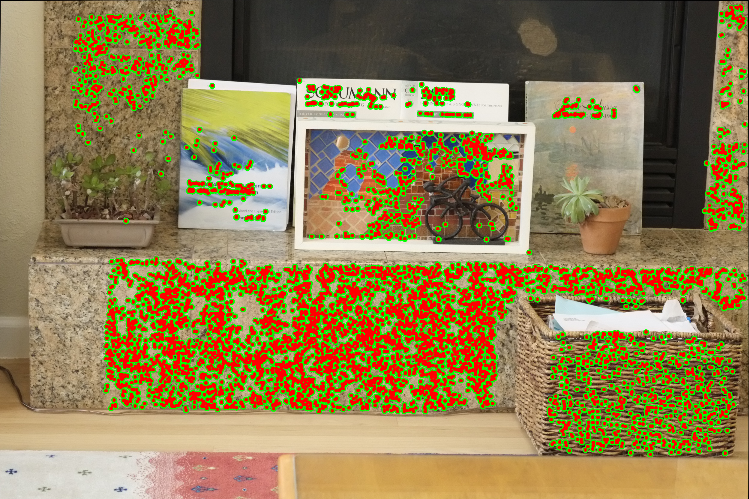
\includegraphics[width=\textwidth]{../Re-projectionPoints}
    \caption{Re-projected point superimposed on the original points.  There is generally a very good correspondence.}
    \label{fig:reproj}
\end{figure}
\FloatBarrier

%====================================Part 4=======================================
\section{Plane Sweeping Stereo}
In this section we calculate a depth map for the combined scene.  First we determine the minimum and maximum depth by looking at the third coordinate of our homogeneous points in the scene.  We find the minimum depth to be approximately 3.36455 and the maximum depth = 3.97782.  We then create 20 equidistant planes and generate a homography for each plane. To generate the homography, we first set the pose matrices of the camera to have the normal to the plane and the depth of the plane in the last row of the equation:
\begin{align*}
	P1 = \begin{bmatrix}
		I & 0\\
		n^T & d_i
		\end{bmatrix}, 
	P2 = \begin{bmatrix}
		R_L^R& {\bf r}^R\\
		n^T & d_i
		\end{bmatrix}
\end{align*}
With this choice of pose matrices the full homography for each depth is calculated as:
\begin{align*}
H = K \left ( P1 P2 \right )_{1:3} K^{-1}
\end{align*}
where the meaning of $\left ( P1 P2 \right )_{1:3}$ is that with this homography we know the last column and last row of the $4 \times 4$ matrix are sent to 0.  The warped images are shown below.
 \begin{figure}[htb!]
    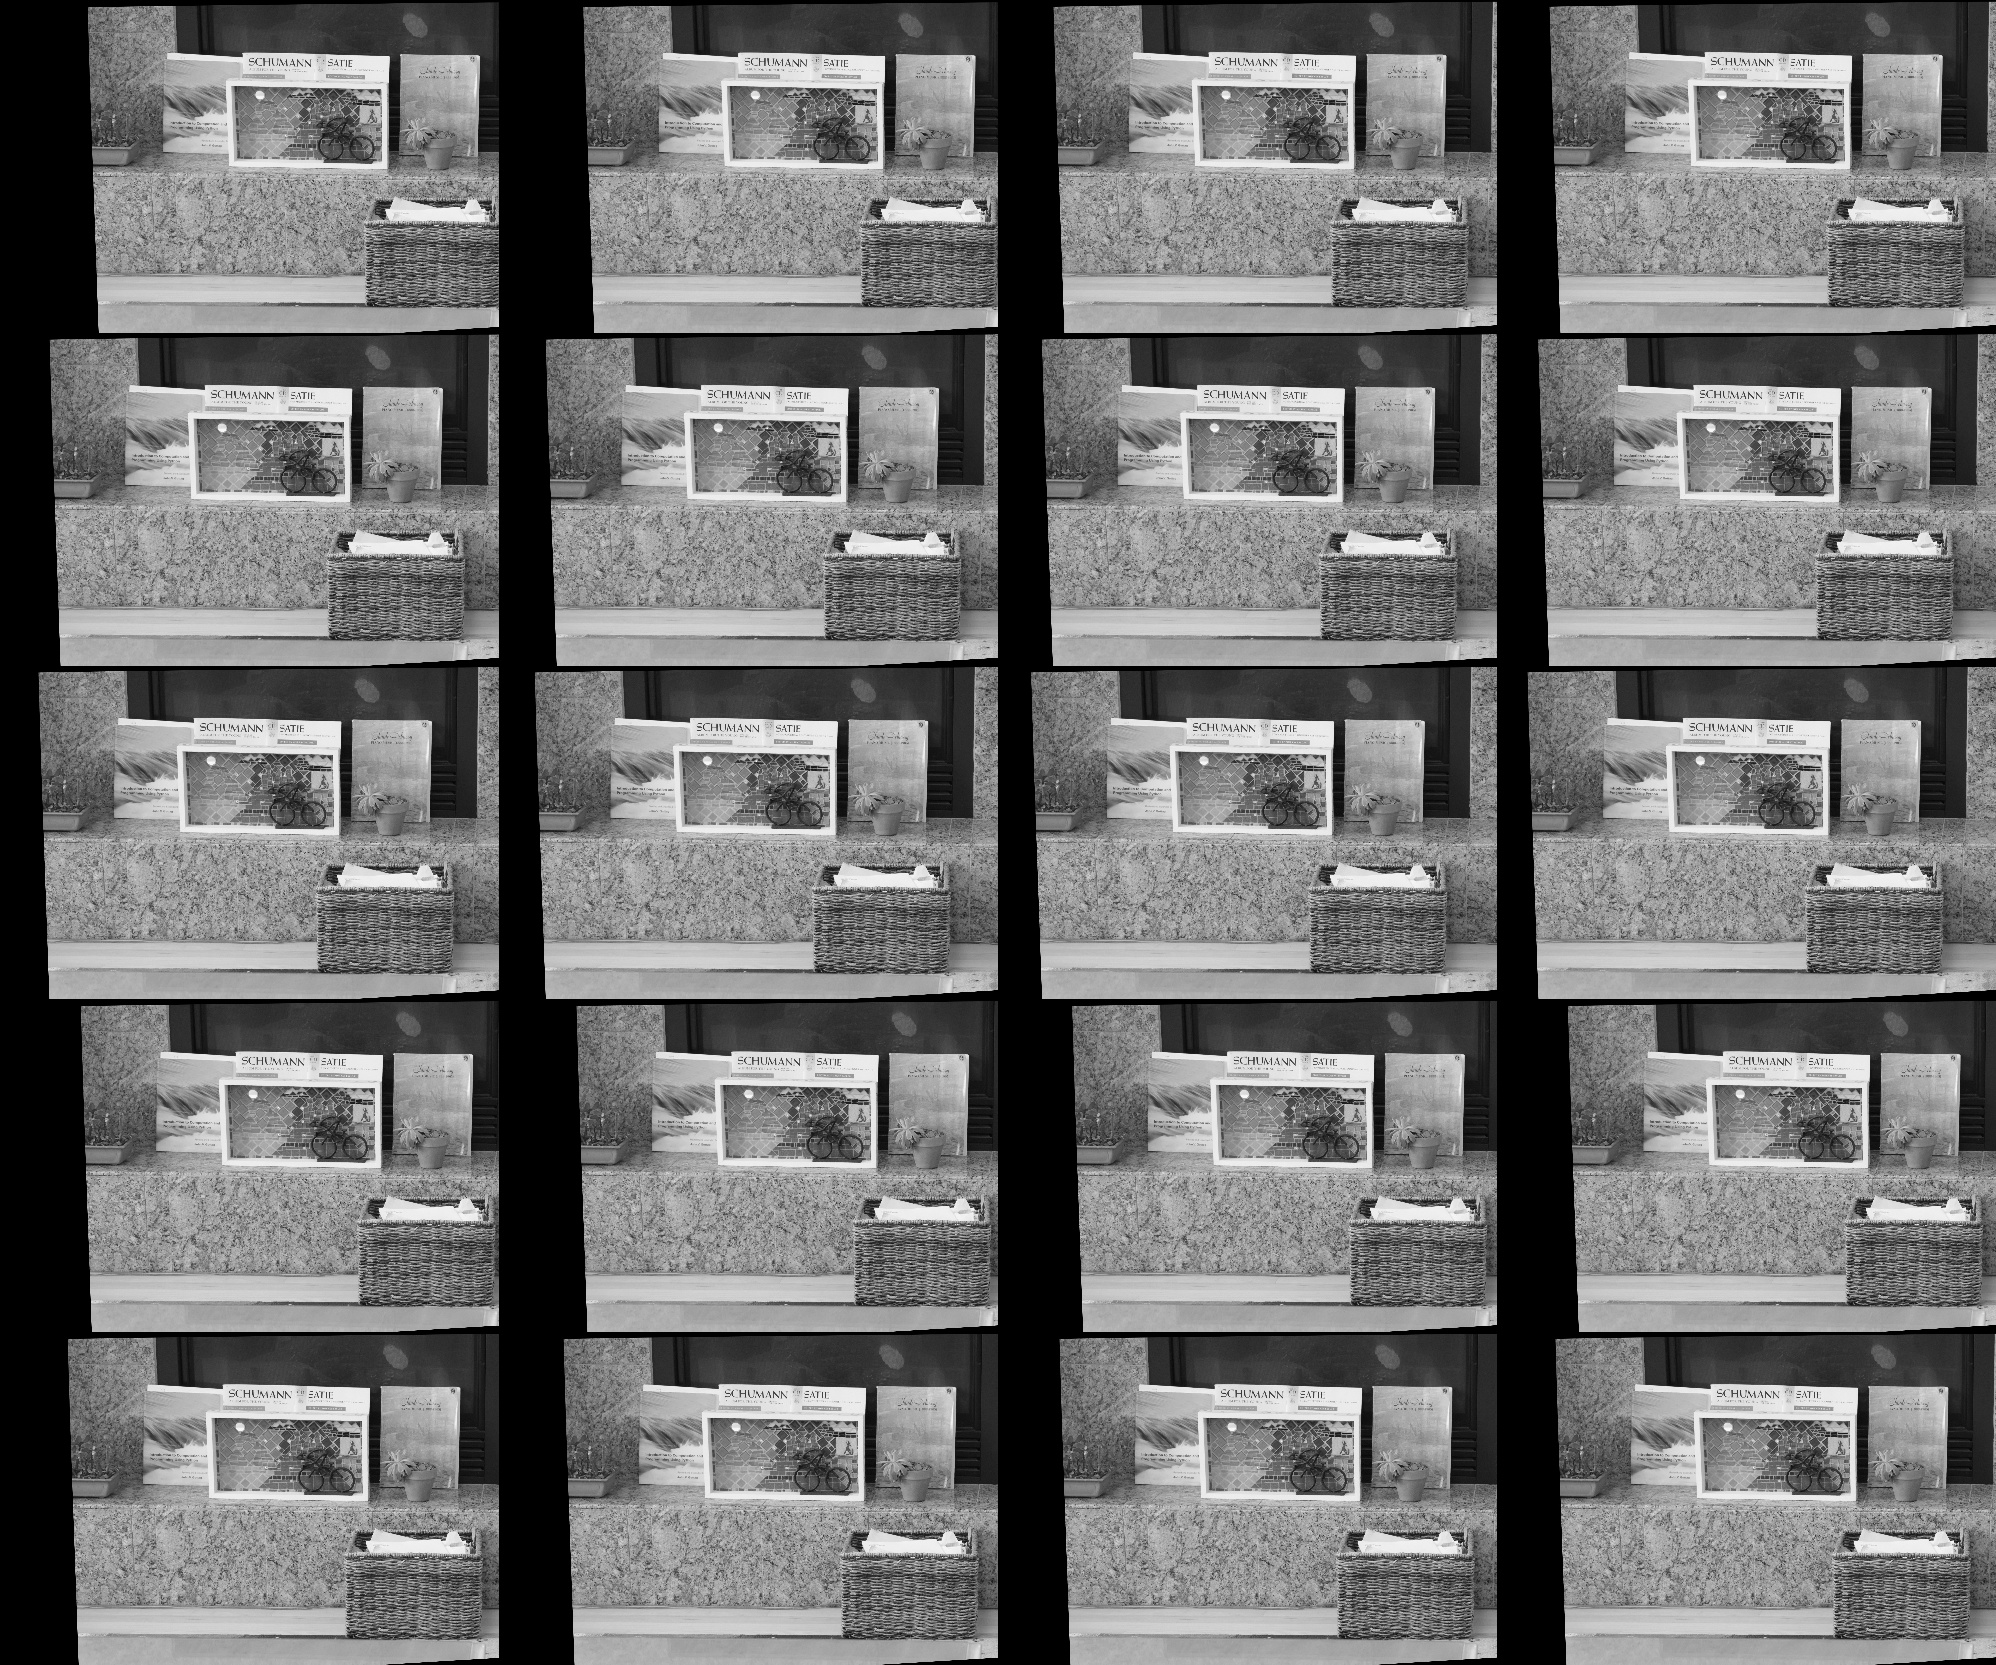
\includegraphics[width=\textwidth]{../ImagesWarping}
    \caption{The twenty warped images after applying the homography that translates each image into the first camera pixel reference frame.}
    \label{fig:reproj}
\end{figure}

It is interesting to see the correspondence of the images as the planes are warped.  Three such images are below in figs(\ref{fig:swpln1},\ref{fig:swpln2},\ref{fig:swpln3})

\begin{figure}
    \centering
    \begin{subfigure}[b]{0.3\textwidth}
        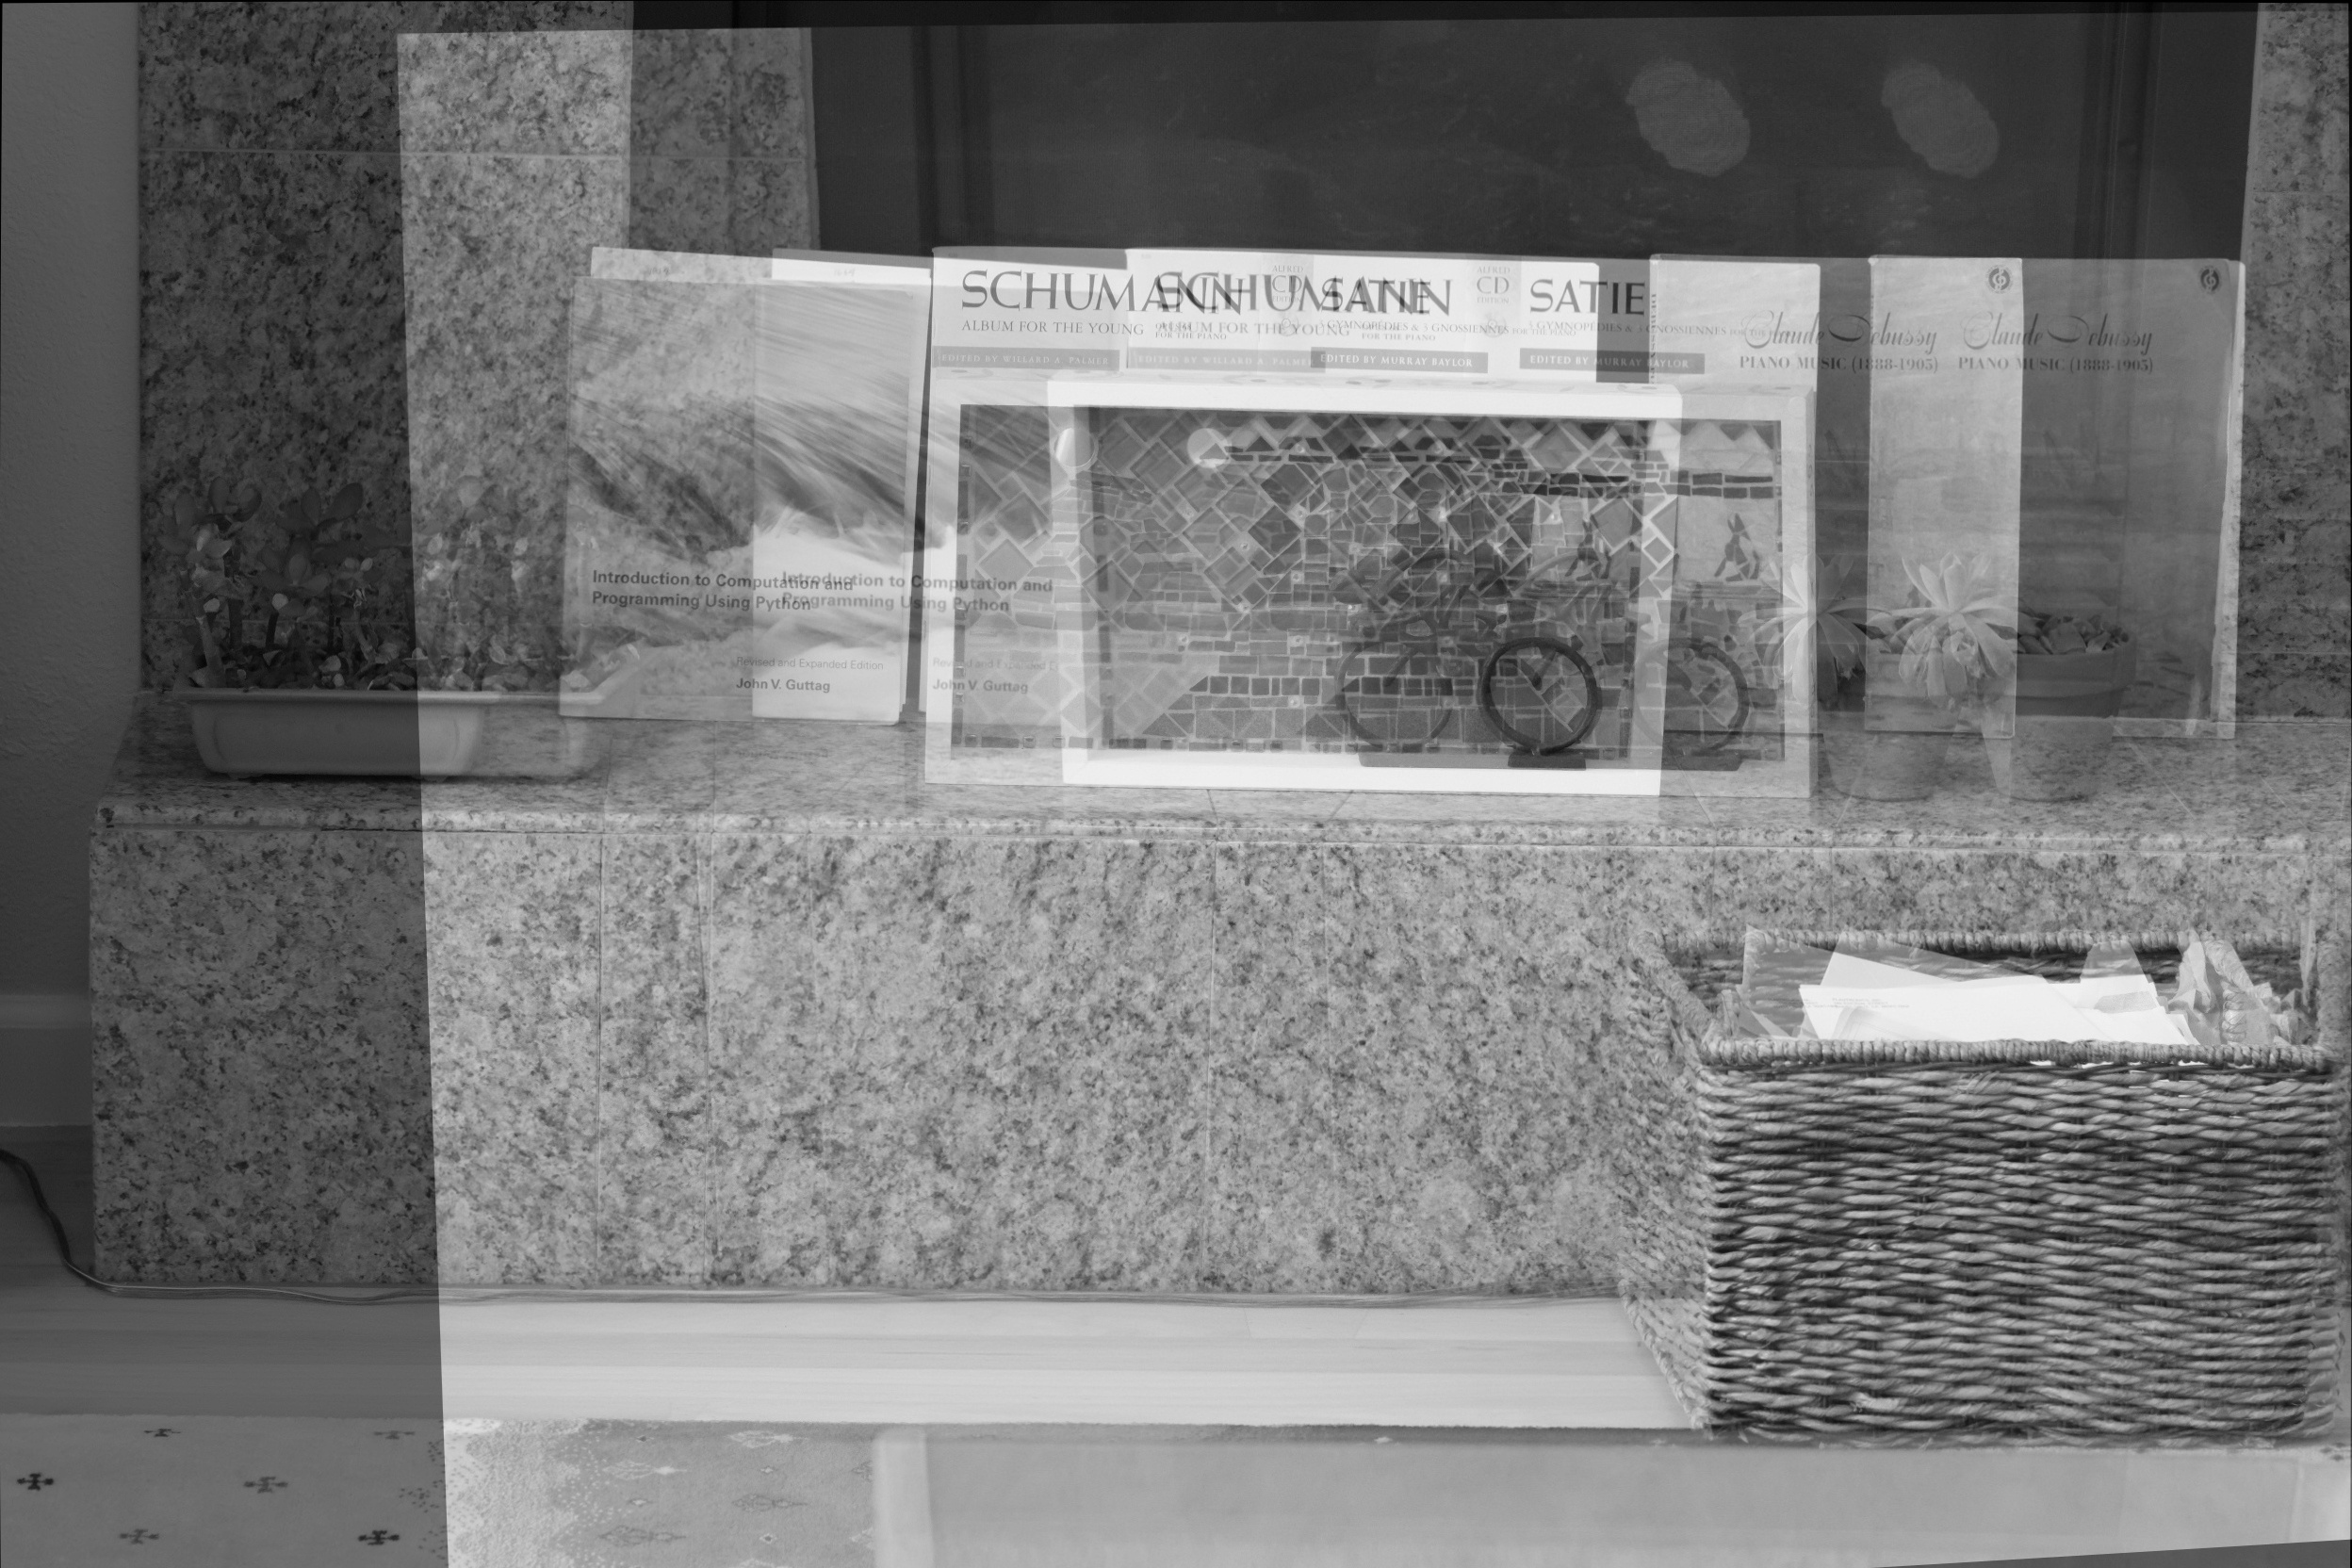
\includegraphics[width=\textwidth]{../Plane_Sweeping/Iwarp1.jpg}
        \caption{The basket in focus.}
        \label{fig:swpln1}
    \end{subfigure}
    \begin{subfigure}[b]{0.3\textwidth}
        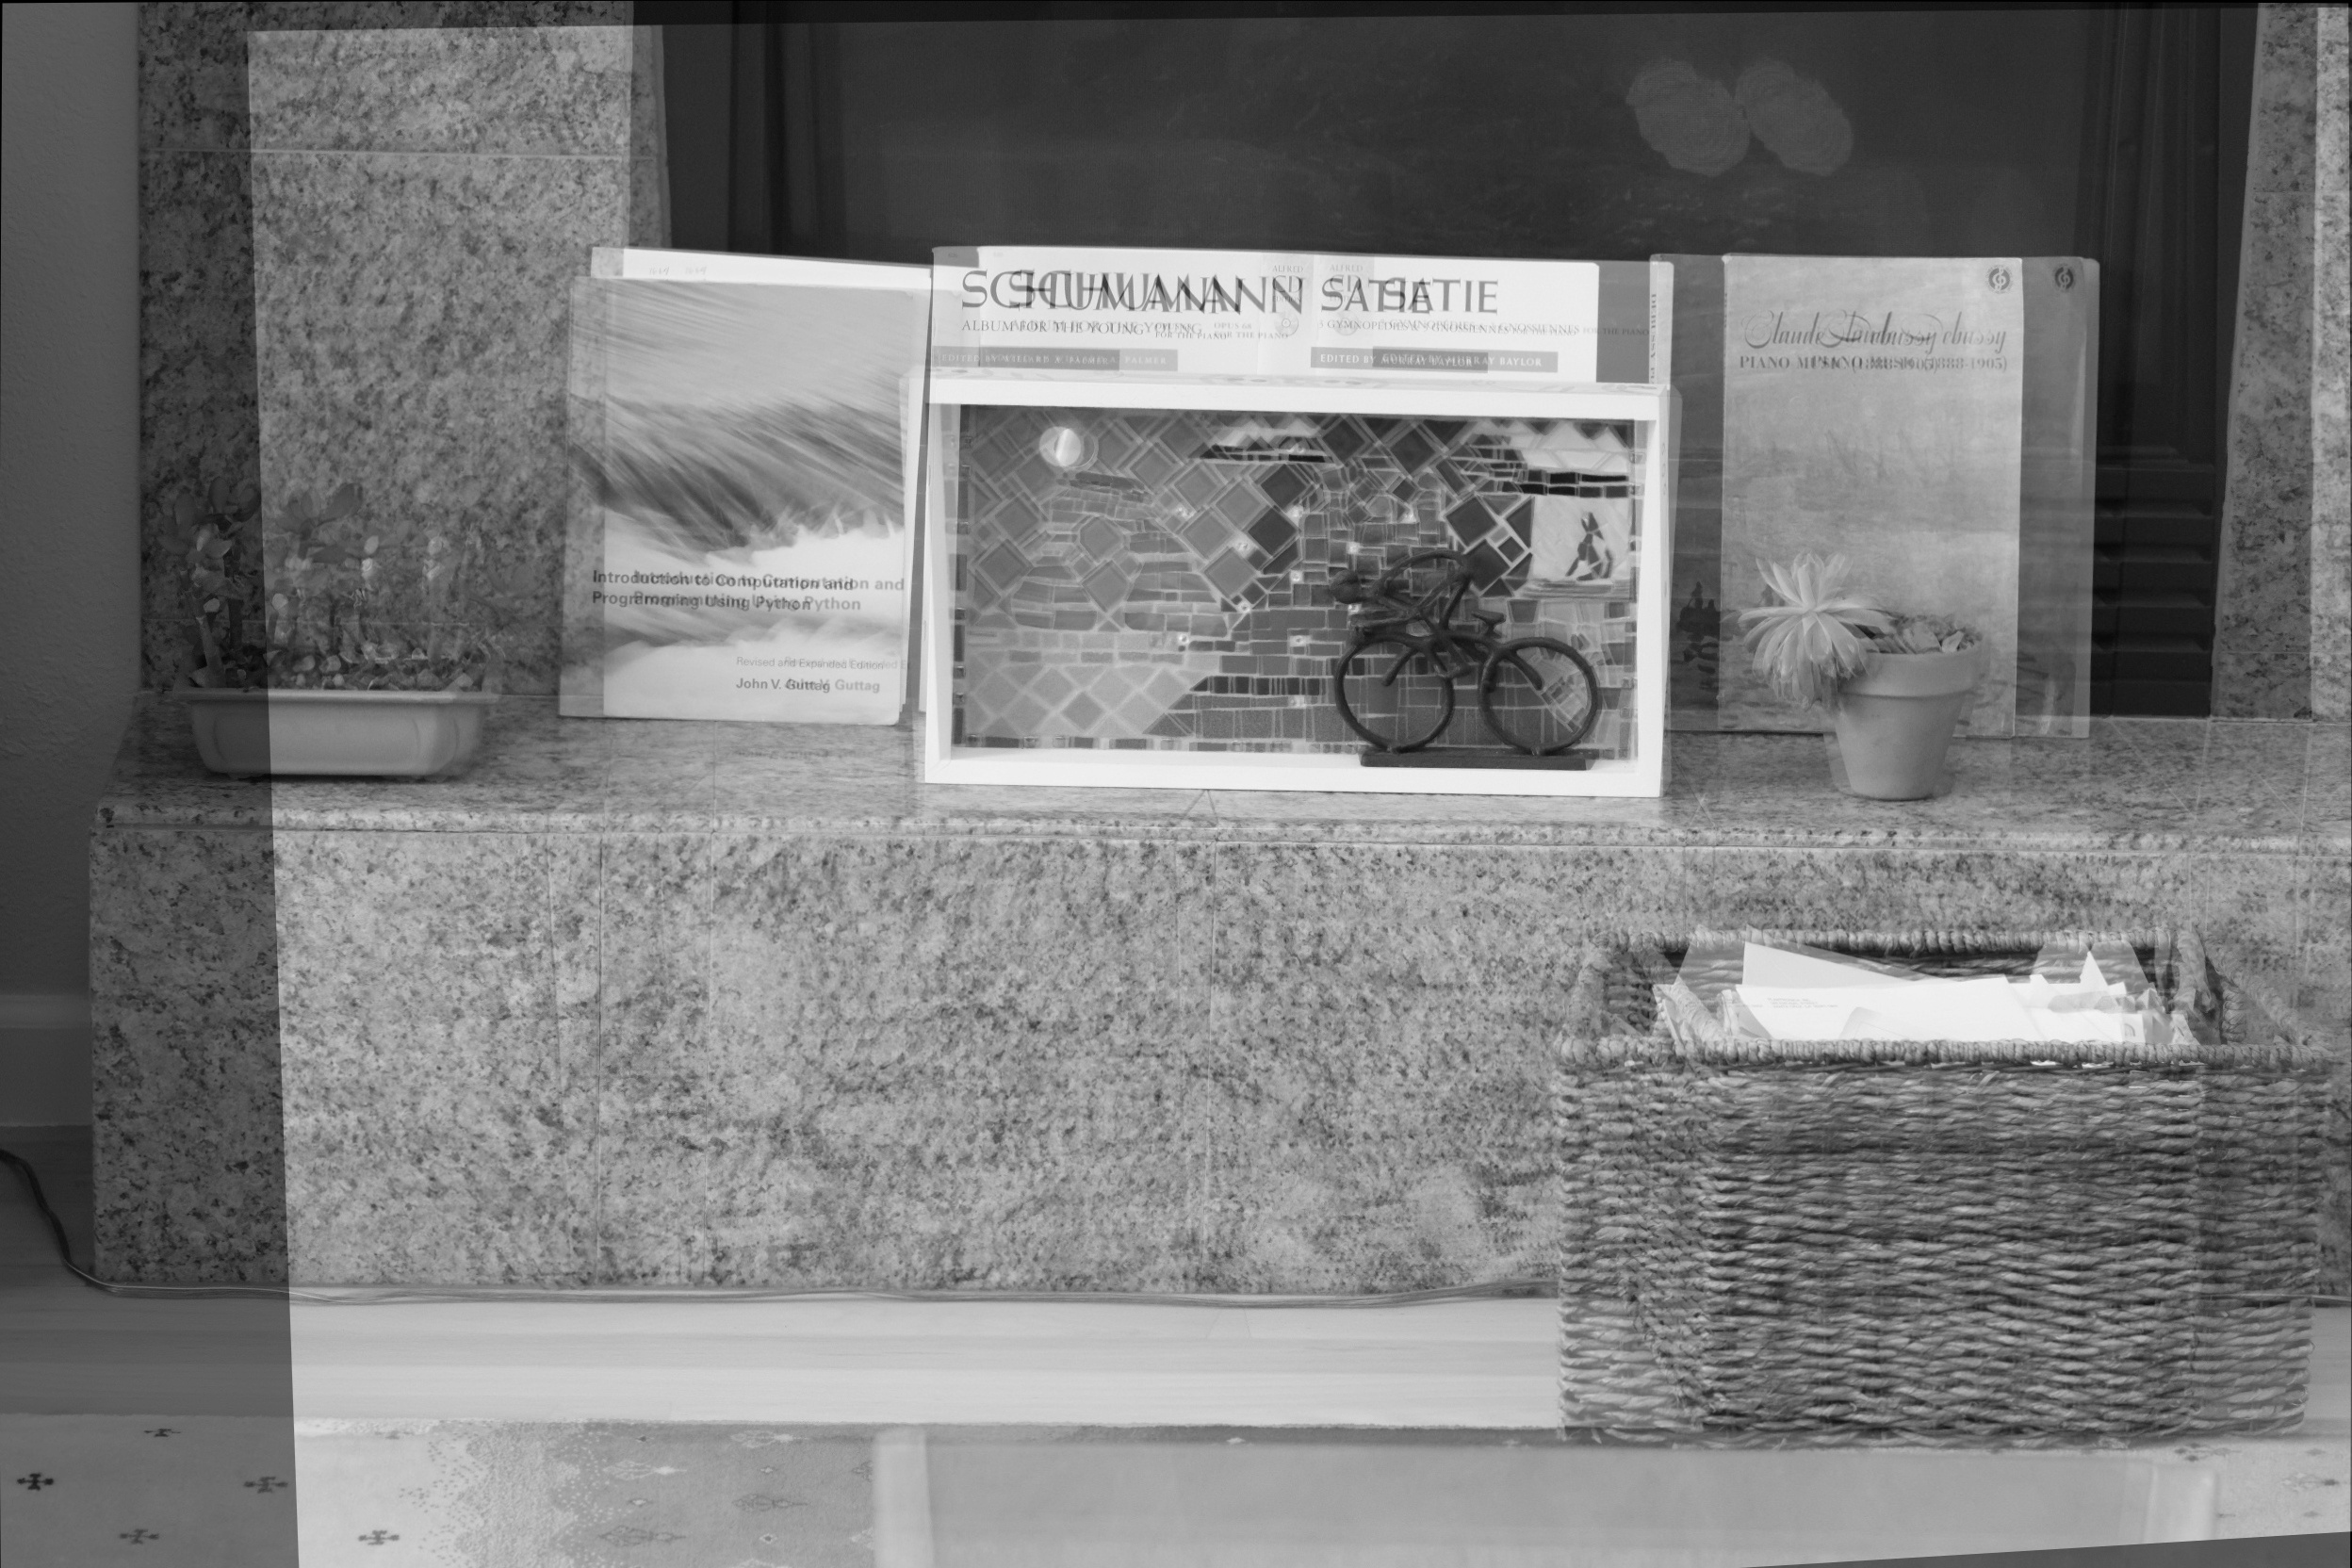
\includegraphics[width=\textwidth]{../Plane_Sweeping/Iwarp11.jpg}
        \caption{Bicycle is now in focus}
        \label{fig:swpln2}
    \end{subfigure}
     \begin{subfigure}[b]{0.3\textwidth}
        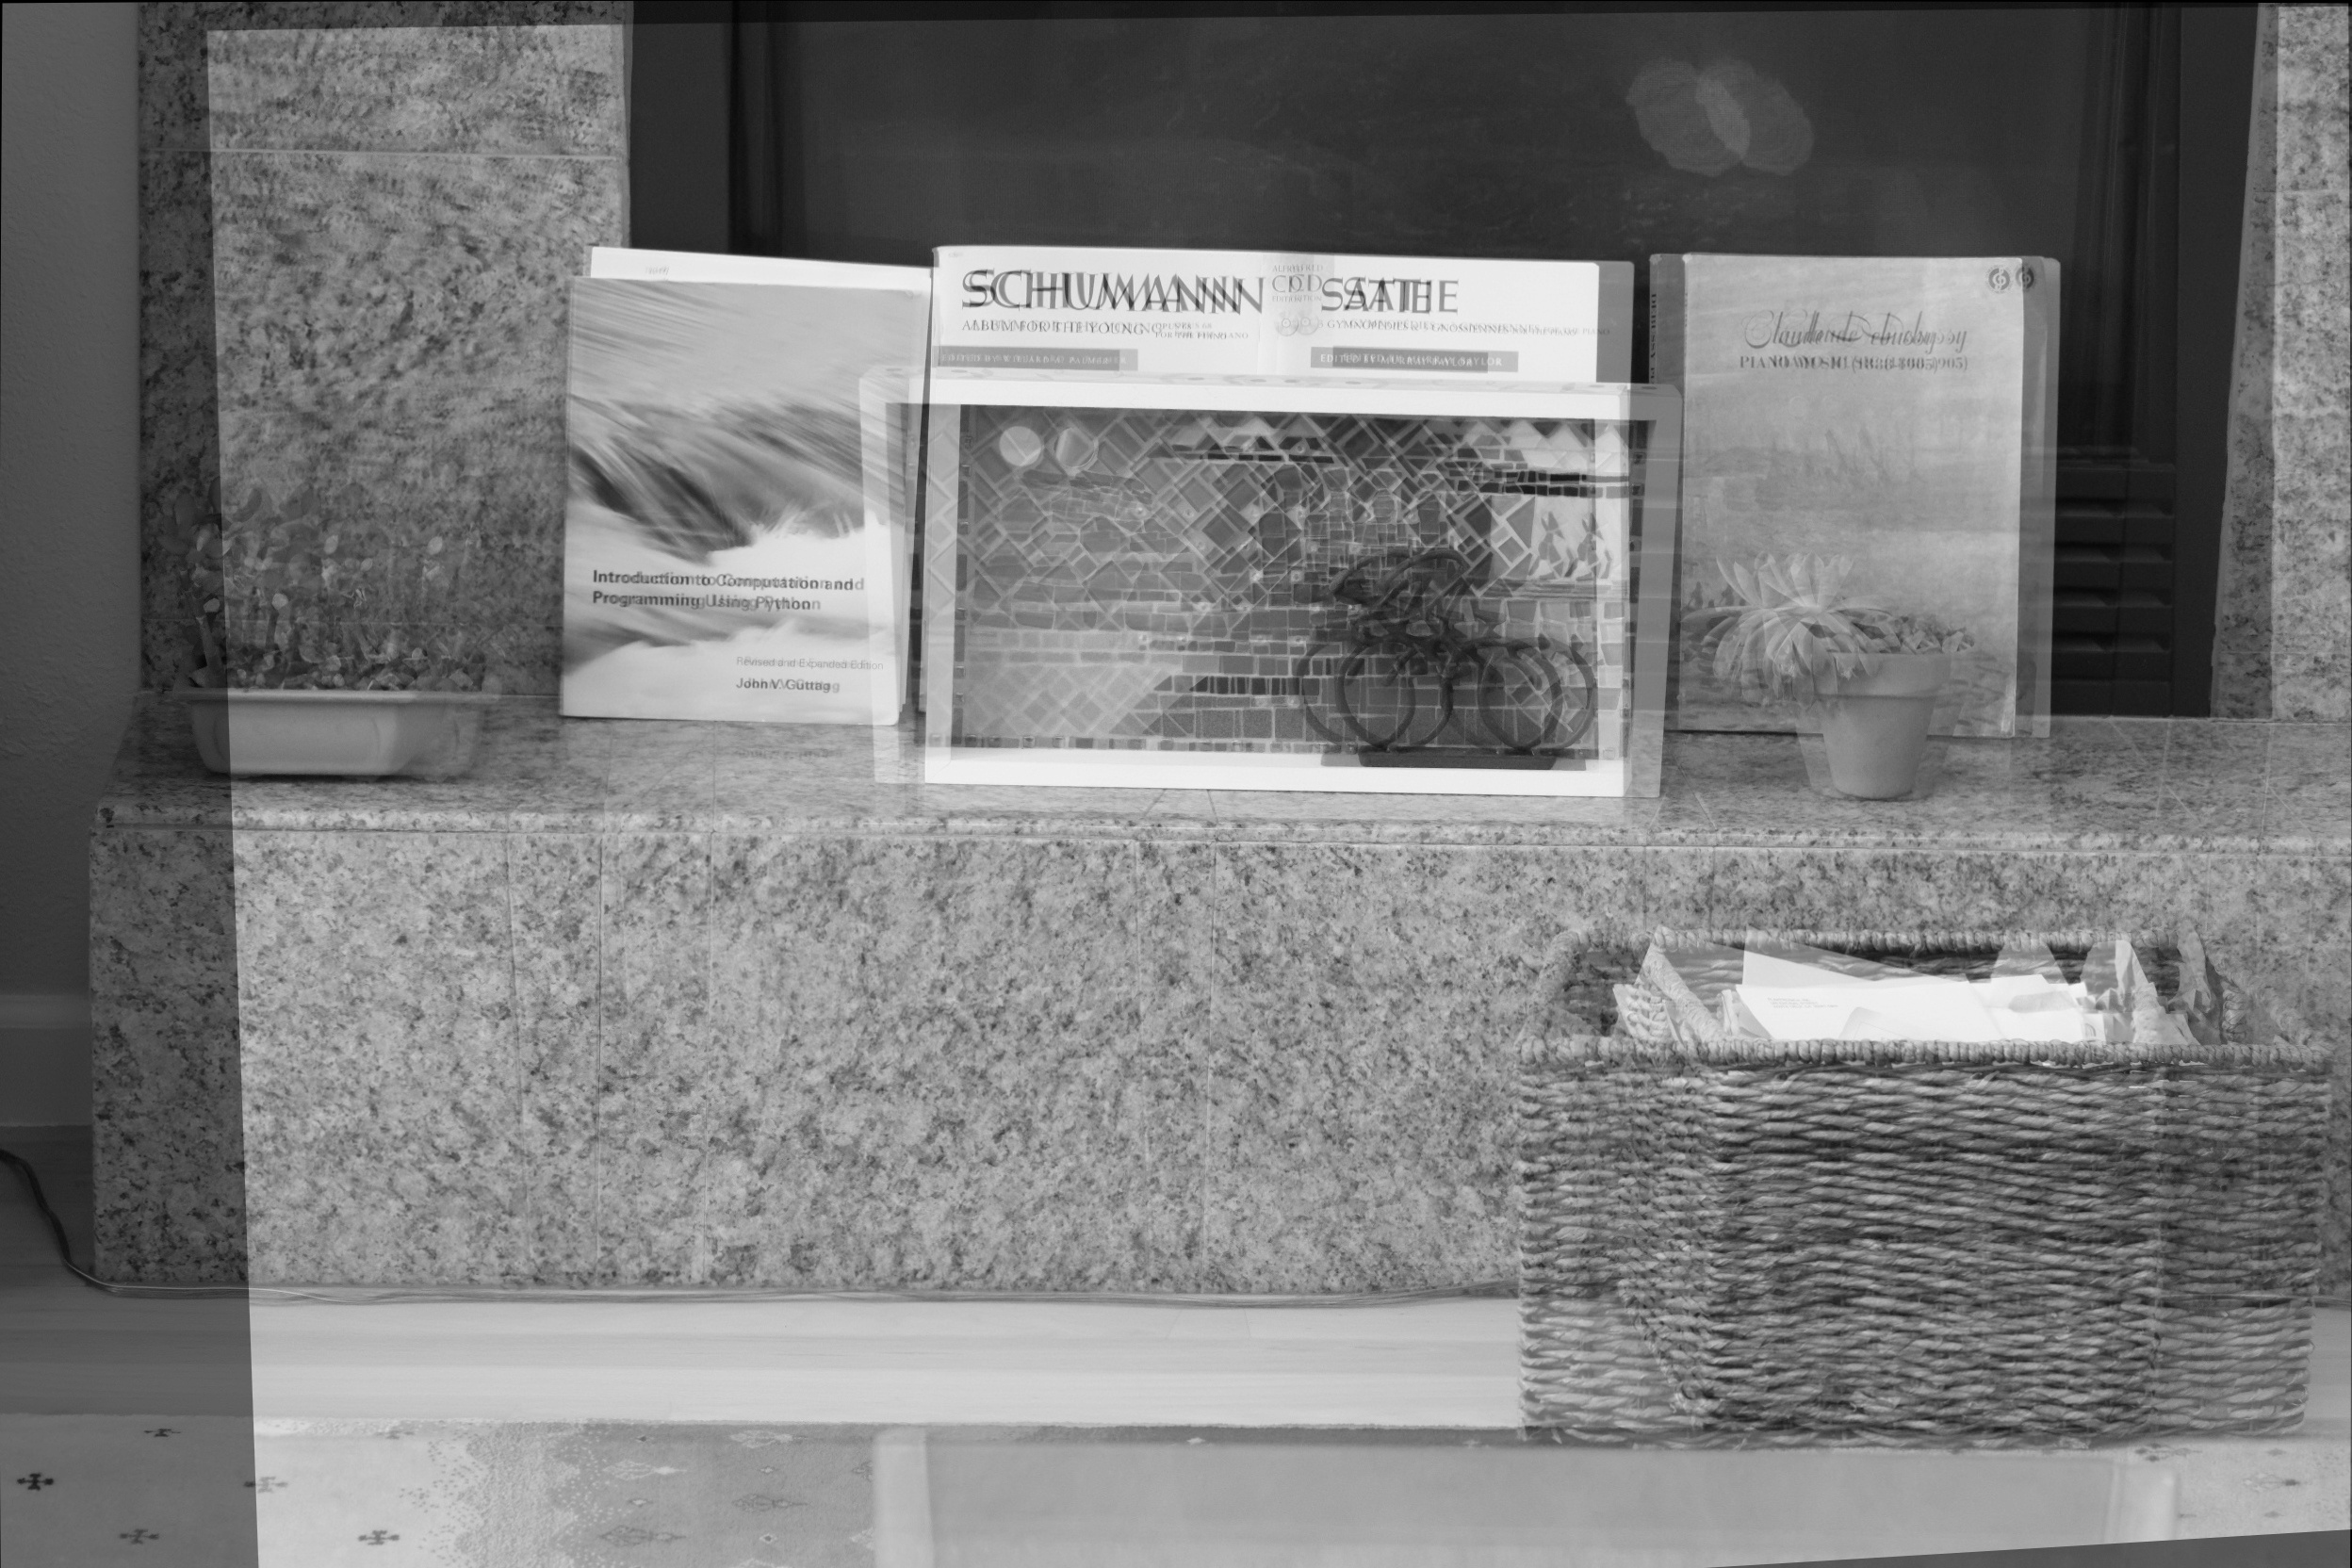
\includegraphics[width=\textwidth]{../Plane_Sweeping/Iwarp14.jpg}
        \caption{The Python text in focus.}
        \label{fig:swpln3}
    \end{subfigure}
\end{figure}

Finally, the depth map itself is calculated.  This is done by first evaluating the absolute difference between each warped image relative to the image 1.  Then  a box filter function from OpenCV is applied to smooth some of the noise in the image resulting from the subtraction.  Finally the minimum absolute difference for each pixel location is computed.  The index of the minimum difference corresponds to the distance of that plane, the value of which is placed in our depth map image at the pixel location in question.  The final depth map is shown in fig(\ref{fig:depth}),  In general the map is reasonable with a large black rectangle on the lower right of the image which is the nearest plane to the camera.  The central rectangle corresponding to the mosaic is also reasonable. The songbooks in the far plane also appear.  The most interesting result, however, is how the front face of the granite stone has diagonal lines running across it.  We hypothesize that this is an artifact due to the speckled pattern of the stone and the filtering function we apply to smooth the image. It appears to alias what should be a well-defined surface.  Perhaps with more manipulation we could resolve this front plane as well. Alternatively, this may be due to the non-parallelism of the camera focal plane and the stone face. 
 \begin{figure}[htb!]
    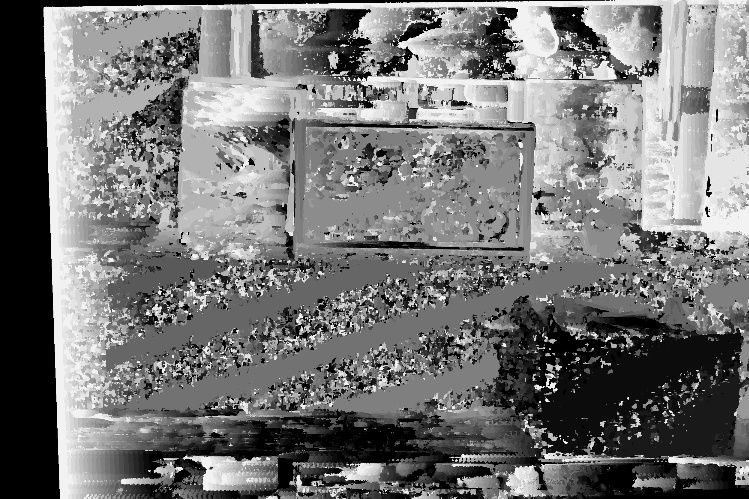
\includegraphics[width=\textwidth]{../ImDepthMap}
    \caption{The computed depth map}
    \label{fig:depth}
\end{figure}
\FloatBarrier
%====================================Conclusions=======================================
\section{Conclusions}
In conclusion, we were able to calibrate a camera using routines  and test patterns provided in OpenCV and test patterns.  With the camera parameters and a sample scene we were able to find matching features and calculate the relative pose of one camera to the other. Knowing the relative orientation and position of the camera allows us to triangulate points in the real world and find their depth, that is how far away from the camera focal plan they lie.  What it doesn't tell us is an absolute distance since all depths are proportional to the baseline vector connecting the optical centers of the two cameras. It is clear, however, that by carefully controlling the location of one camera relative to another a true stereo camera could be constructed.





\end{document}